\documentclass[cmbright,fleqn,referee]{envauth}

%%%%% AUTHORS - PLACE YOUR OWN MACROS HERE %%%%%

\def\bSig\mathbf{\Sigma}
\newcommand{\VS}{V\&S}
\newcommand{\tr}{\mbox{tr}}

\received{00 Month 2013}
\revised{00 Month 2013}
\accepted{00 Month 2013}

\newtheorem{theorem}{Theorem}

\usepackage{natbib,upgreek}
\usepackage{bm}
\usepackage{comment} % to comment out large sections of text
\usepackage{float}
\usepackage{multirow}
%\usepackage[nolists]{endfloat}

\usepackage{color}
\newcommand{\hilight}[1]{\colorbox{yellow}{#1}}

\runninghead{R.~Joy et al. }{BHM for Animal Behaviour}

\begin{document}

\title{Modelling Marine Animal Behaviour using a BHM Model}

\author{R. Joy\affil{a}\corrauth\, M. Dowd\affil{b}, B. Battaile\affil{c},  A. W. Trites\affil{c},  R. Routledge\affil{a}, P Lestenkoff}

\corraddr{R. Joy, Department of Statistics and Actuarial Science, Simon Fraser University, 8888 University Drive, Burnaby, British Columbia, V5A 1S6, Canada. E-mail: rutherfordjoy@gmail.com}

\address{\affilnum{a}Department of Statistics and Actuarial Science, Simon Fraser University, 8888 University Drive, Burnaby, British Columbia, V5A 1S6, Canada. \\
\affilnum{b} Department of Mathematics and Statistics, Dalhousie University, 6316 Coburg Road, PO Box 15000 
Halifax, Nova Scotia, B3H 4R2, Canada
\affilnum{c} Marine Mammal Research Unit, Fisheries Centre, University of British Columbia,2202 Main Mall, Vancouver, BC, Canada V6T 1Z4}

\begin{abstract}

\hilight{Will rewrite after we are done, to reflect new and more general emphasis} \\

The population of northern fur seals ($Callorhinus$ $ursinus$) in the Pribilof Islands, Alaska has declined dramatically during the past 35 years. Arresting the decline of the species requires an understanding of their foraging behaviour at sea and is particularly important for those adult females whose foraging success is also linked to pup survival. We capture behaviour patterns of a set of tagged female northern fur sells by relating an autoregressive movement model to the numerical properties of the state space. The at-sea behaviour states were then matched, spatially and temporally, to a set of environmental variables, some of which were averages that represented the oceanic conditions over a large spatial area. The mismatch of scale between fur seal behaviour and the environmental variables was accounted for by modeling the errors associated with these covariates in a Bayesian hierarchical regression framework. Using this approach, we were able to link together northern fur seals that went to disparate regions of the eastern Bering Sea, with widely variable information about their underlying environmental fields into a single model. This application of a hierarchical model relates changes in identifiable behavioural states of the northern fur seal to changes in the Alaska commercial groundfish industry over a 24-hour foraging cycle. \end{abstract}

\keywords{Northern fur seal; Mulitnomial; Bayesian hierarchical model, Error-in-covariates; \\Diel pattern; Walleye Pollock}
\maketitle

% ----------------------------------------------------------------------------------------------------------------------------------------------- %
% start of document
\section{Introduction}
\label{s:intro}

\hilight{MD will rewrite Intro}. \\ 

The population of northern fur seals in the Pribilof Islands, Alaska has declined dramatically during the past 35 years, and continues to decline without any obvious reason yet identified (Towell et al. 2006). Arresting the decline of the species requires an understanding of the foraging strategies of the northern fur seal (Antonelis et al. 1997), particularly for those adult females whose foraging success is also linked to pup survival. The relationship between lactating northern fur seal movement and habitat is shaped by foraging success and the physiological constraints of feeding a stationary pup left on a beach at its natal rookery. Understanding the relationship between movement, behavior and environment is a critical part of understanding population processes (Bowler and Benton 2005% in Patterson et al. 2009, pg 1118
), and has been identified as one of the highest-level priorities by the northern fur seal conservation plan (NMFS 2007). 

%Success of foraging is dependent on northern fur seals finding sufficient prey on their foraging trips through a dynamic ocean environment. Previous radio and satellite telemetry studies of northern fur seals on the Pribilof Islands have shown that feeding areas are between 160-200 km offshore and as far as 370 km from St. Paul Island (Loughlin et al. 1987). 

%Despite the limitations of being tied to a rookery during the pupping season, the foraging routes from the Pribilof Islands appear to radiate outward with little formal pattern, but with some rookeries displaying a rookery-specific directional bias (Robson et al. 2004, Call et al. 2008). Past telemetry has shown, in some individuals, a within-season foraging route fidelity, with greater weight gains in those females that followed this strategy (Call et al. 2008). 

%Physical and biological features undoubtedly influence northern fur seal movements, but the identification of the extent of these influences remains limited (Ream et al. 2005, Kuhn et al. 2010). In particular, our understanding of the overlap between the commercial fishery and active foraging of northern fur seals remains poorly understood. 

%Analyses of satellite-linked dive depth data (TDR/SDR tags) to physical and biological features, have provided some understanding of at-sea dive behavior of fur seals, but the horizontal resolution of the data has been too coarse to link to fine-scale foraging preferences. 

%Others have correlated northern dive depth to bathymetry (Antonelis 1997, Call et al. 2008) and lunar cycle (Ream et al. 2005). Foraging behaviour has been linked to thermocline depth and surface fronts (Kuhn 2011, Nordstrom et al. 2013), and denser prey patches found off-shelf (Benoit-Bird et al. 2013b).  These results represent an important advance in our understanding of at-sea ecology; however, 

%Therefore, examining fine-scale 3-dimensional movement and behaviour in the context of the physical and biological environment the animals encounter should help us to better understand fur seal ecology and survival.

%to gross oceanographic features (e.g. Loughlin et al. 1999, Call et al. 2008), such as the continental shelf break to the west of the Pribilof�s (Goebel et al. 1991, Robson et al. 2004, Sterling and Ream 2004). 


%Stomach contents collected in the 1960�s and 1970�s and scat collected starting in the 1990�s have consistently shown that the dominant prey in fur seal diets is the commercial groundfish, walleye pollock (Perez and Bigg 1986, Sinclair et al. 1994, Zeppelin and Ream 2006, Zeppelin and Orr 2010). Northern fur seal satellite data has so far linked at-sea locations. Bengtson et al. (1985) used coarse telemetry methods to locate female fur seal feeding sites to assess the interaction of fur seals with commercial trawl fisheries and found an association along the continental shelf. 

%However, 3-D track reconstruction that would couple the fine-scale spatial overlap of the commercial groundfish fishery to fine-scale foraging activity, would help us to better understand fur seal ecology and survival. 

%None of the models to date have considered the uncertainty in the acquired set of covariates. Yet the data uncertainty in modelling behavioural response to environmental covariates is omnipresent and unavoidable. The hierarchical model proposed in this chapter is ideal for incorporating uncertainty at all levels. As data quality improves, as well as our understanding of the underlying environmental processes, these methods are flexible enough to allow for better, more mechanistic, and less error-prone models of behaviour. 

%of 3-dimensional movement into the classification of behaviour, and the construction of a flexible framework for drawing inference about behavioural responses to changes in the at-sea environment. We choose to apply this hierarchical framework to a data set of eleven instrumented northern fur seals and analyze each animal's tag-data from her at-sea voyage through the Bering Sea.   

%3-D
Analysis methods have been hampered until recently by difficulties in reconstructing the three-dimensional foraging tracks through the oceanic environment (Harcourt and Davis 1997). Movement is a complex 3-dimensional process that does not always simplify into lower dimensions, yet there is mounting evidence to demonstrate the potential perils of inferring animal behaviour based on horizontal trajectories alone (e.g. McClintock et al. 2013 and references therein). Methods that calculate horizontal straightness indices (e.g. area restricted search: ARS) have found this poorly correlates to feeding behaviours (Austin et al. 2006, Weimerskirch et al. 2007). Another metric measuring passage time through a horizontal region of fixed radius (e.g. first passage time: FPT) has been linked to covariates but suffers from the confounding of slow speeds due to rest behaviours, and fast speeds with tortuous paths taking similar times to traverse a similar radius. Other methods based on depth (e.g. Gentry et al. 1986, Goebel 2002) are dependent on arbitrary depth descriptions. The methods used here take advantage of recent advances in 3-D bio-logging technology and use movement models based on processes that describe dive types in a mechanistic way. This approach to classifying behaviour links the vertical dimension to the horizontal spatial field that describes the environment in which the behaviour is observed. The framework is a flexible, analytical method for extracting more out of the increasing wealth of information from recent advances in bio-logging technology. We show how to incorporate this information into understanding the environmental factors influencing at-sea behaviour.  

% Error-in-Cov
The environment undoubtably influences northern fur seal behaviour, but identification of the extent of these influences is limited, and remains poorly understood (Ream et al. 2005).   Linking behaviour to changes in the environment at the landscape level is important in understanding the processes that limit at-sea success in the Bering Sea. The main barrier to developing models addressing these landscape level questions is the vast difference in scale between the at-sea behaviour of the individual seal and the oceanic environment through which that fur seal passes. The environment is typically only observed incompletely and with large and unknown amounts of measurement error and data uncertainty. As well, the environment can only be approximated by combining various data sources, often at very different scales. These issues can represent a significant amount of modelling uncertainty, and this is true of any analysis that aims to link animal movement to the spatial environment. The amount of uncertainty in the data can depend on a number of factors. For example, spatial data can be collected from ships   running transects across time and space, or can be derived from remotely sensed satellite data. Each data collection agency usually has its own way of pre-processing the data to account for limitations of the sampling method. 

The general approach to hierarchical modelling can be considered as a large set of stochastic formulations that include many popular models such as random effects models and generalized linear mixed models, and are flexible enough to solve a variety of inference problems (e.g. Gelman et al. 2004, Chapters 5, 15, and references cited therein). We introduce in this paper a hierarchical Bayesian model as a means to account for multiple sources of uncertainty in the measurement and quantification of the fur seal's at-sea environment.  We develop a Bayesian hierarchical model for processing 3-D movement models and the effects of covariates for multiple individuals motivated by the problem of (i) processing a dataset collected from satellite-linked, archival tagged female northern fur seals with pups, and (ii) understanding their at-sea behaviour in response to changes in the environment. We will formally acknowledge the randomness in both seal behaviour and the environment process by building a hierarchy of conditional models to describe the complexity of our data and the process that generates animal behaviour (Cressie et al. 2009).
We do not set out to identify which sections of the Bering Sea might be of conservation priority with respect to foraging hotspots, and therefore have not approached this as a spatial problem.  Our goal is to understand if there was something in the variable field through which the fur seal swam, that influenced the observed fur seal's behaviour. %Specifically, we reconstruct the 3-dimensional foraging tracks of a set of northern fur seals using satellite linked archival tags, and relate the changes in movement along the tracks, to changes in their at-sea environment. 
Our specific goals are:
\begin{enumerate}
\item To use archival tag technologies recording movement at scales of seconds, in conjunction with coarse location data from Argos satellite transmitting tags, to understand how lactating fur seals partition their time between different identifiable behaviours such as active feeding, exploratory diving, and non-feeding behaviours such as sleeping, resting, grooming or surface transiting.  
\item To understand how these identified behaviours can be linked to their at-sea habitat and used to understand how physical and biological factors influence their behaviour. 
\end{enumerate}
 
While the primary focus of this paper is on the behaviour of northern fur sells at a rookery site on the Pribilof Islands, it is important to emphasize that the methodology is adaptable. As data quality improves, as well as our understanding of the underlying environmental processes, these methods are flexible enough to allow for better, more mechanistic, and less error-prone models of behaviour. As well, this framework will allow for the characterization of the relationship of the behaviours we classified, but also of other behaviours and other descriptors of pelagic habitat and foraging success, and presumably, of other marine predators. 

%This paper is structured as follows. A set of vertical movement data is introduced, a suitable movement model is proposed, and a general methodological approach is outlined in Section~\ref{s:METHODS} with details on the application of the methodology. Results are given in Section~\ref{s:RESULTS}. A discussion follows in Section~\ref{s:DISCUSSION}.



\section{Data}
\label{s:METHODS}

\hilight{ general lead in statement should go here} 

\hilight{ note that we introduce data set/case study first = concrete anchor} 


\subsection{Instruments} \label{s:INSTRU} 
During the 2005 and 2006 breeding seasons, 18 lactating northern fur seals were captured at Reef Rookery on St. Paul  Island (57.18$^\circ$ N, 170.27$^\circ$ W; 5 in 2005, 13 in 2006).

Three different tag technologies were employed in which all instruments were attached mid-dorsally using methods described in Boyd and Coxall (1992). The first of these tags was a dead-reckoner tag (Driesen \& Kern GmbH, Bad Bramstedt, Germany). The dead-reckoner tags were programmed to collect data at 2-second or 5-second intervals for the full length of the foraging trip. Two of the 2005 tags were set to sample at 5-second intervals, and the remaining 2005 and all 2006 tags were programmed to sample at 2-second intervals. The dead-reckoner was a 10-channel logger with a 32 MB flash memory that recorded time, depth, speed (using a swim paddle system), temperature, light, pitch, roll, compass heading (in three-dimensions), and body orientation (belly up or belly down). 

The second tag attached was an ARGOS (Platform Transmitter Terminal or PTT) satellite transmitter (Spot5, Wildlife Computers, Redmond, Washington, USA), recording latitude and longitude to recalibrate dead-reckoner route calculations from cumulative errors associated with ocean drift. 

The third tag attached was a VHF radio transmitter (A2920 Glue On, Advanced Telemetry Systems, Isanti, Minn., USA), to allow the animals to be relocated when they returned to the rookery. All females were recaptured to remove the tracking devices and retrieve the data series logged from their at-sea foraging trips. \\

\subsection{Track Reconstruction}
\label{s:RECON}
The 2- and 5-second resolution data recorded on the dead-reckoner tags and the Argos transmitters were integrated to link swimming position to the satellite location data (Mitani et al. 2003). The 3-dimensional fur seal track was calculated using the dead reckoner channels that recorded compass bearing, depth, and speed-through-the-water to calculate the direction and horizontal speed over the water surface for each female. We pre-processed the tag's speed channel to correct for cumulative errors due to bias in the speed paddle's position. We identified zero-speed periods (sleeping) using short (13 minute) time windows with near-zero variance, and used a linear interpolation to re-zero speed (Figure \ref{f:CorrSpeed}). Each foraging track was then corrected for errors associated with ocean drift by matching times of the two tags, and forcing the dead-reckoner track to lie between the (assumed to be correct) Argos locations. This was done by translating the dead-reckoner track into polar coordinates, rotating the angle of movement, and rescaling the radial coordinate to match the direction and great circle distance between consecutive Argos locations (Figure \ref{f:recontrack}). This resulted in a 2- or 5-second resolution track reconstruction that infills between the Argos satellite locations. These high-resolution track reconstructions allowed a space and time linkage between the environmental conditions encountered and the behavioural response of each northern fur seal. We trimmed each female's data record to include only those data in which she was at sea. The trimmed tracks ranged from 90,000 to 480,000 3-dimensional data records per animal (Figure \ref{f:MAP3}).\\

\begin{figure}
 \centerline{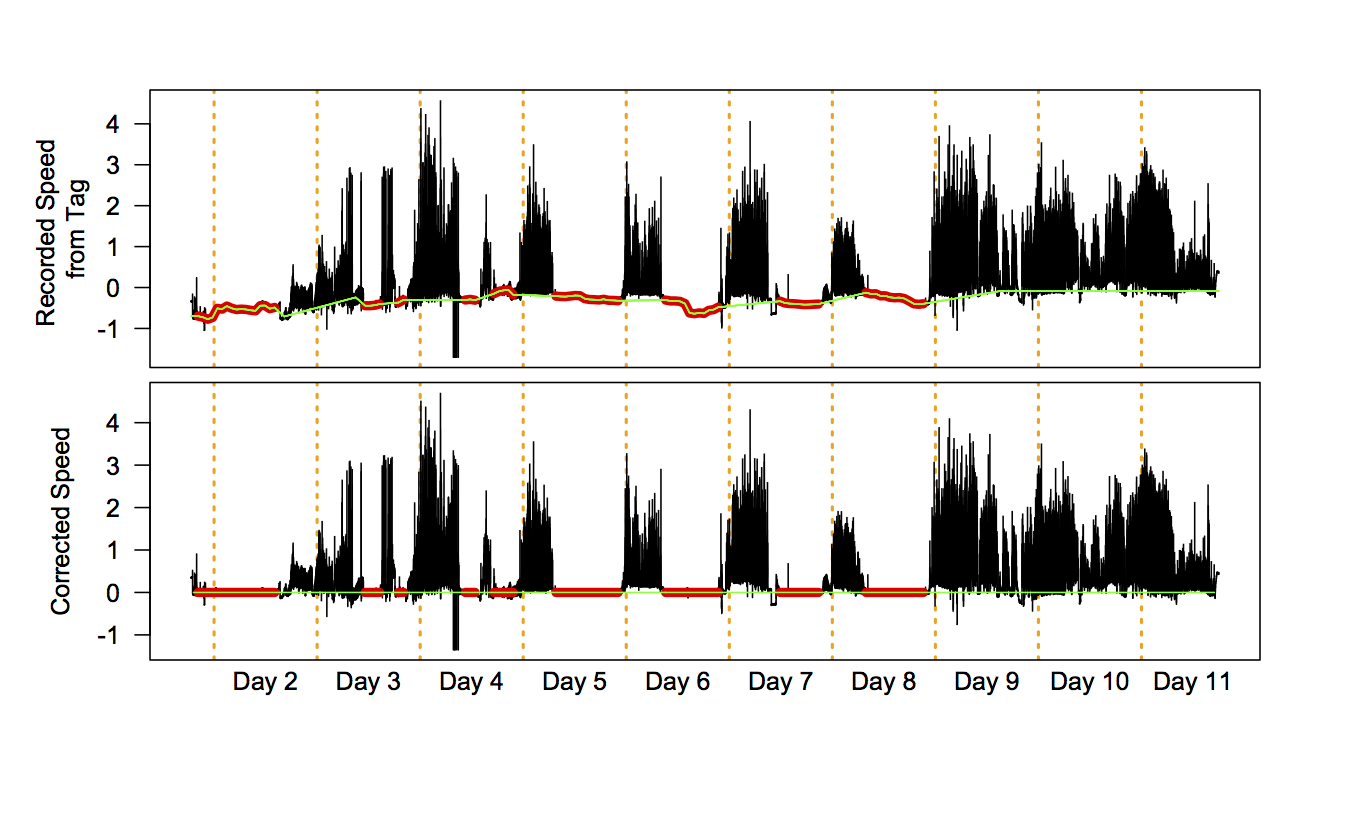
\includegraphics[width=7.25in]{CorrSpeed.png}}
\caption{The entire raw data record for 1 female northern fur seal from the dead-reckoner's $speed$-$through$-$the$-$water$ channel, before and after the data series is  corrected for drift from zero speed. Speed is measured as speed through the water, and not over the ocean bottom, and is a tentative, approximate measure until an updated, satellite-based location can be obtained along the track. Changes in day (at midnight) are represented in this figure by the dashed vertical lines. Length of data series depicted here is 482,400 elements, and we refer to this track in the text as ``Track 3''.}
\label{f:CorrSpeed}
\end{figure}

\begin{figure}
 \centerline{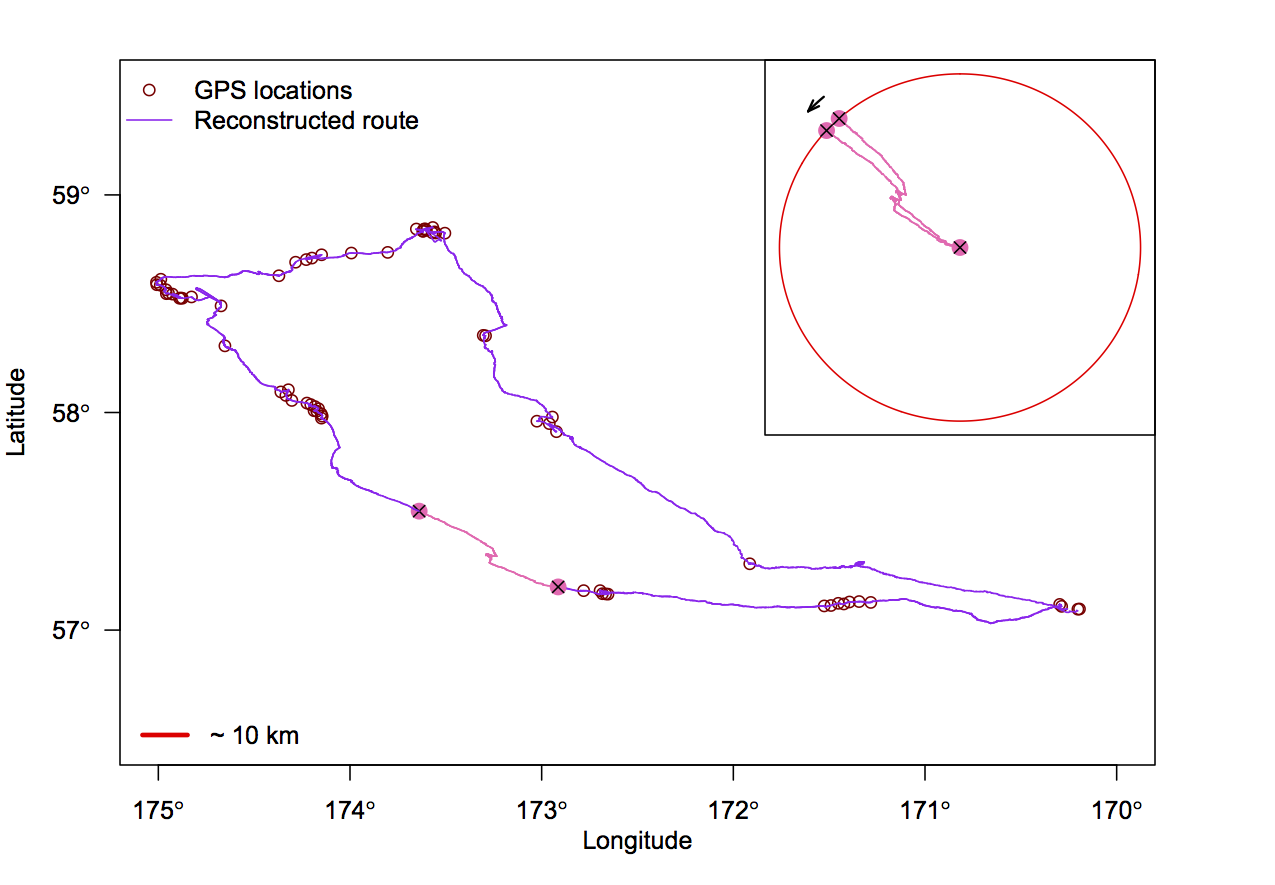
\includegraphics[width=7.25in]{recontrack.png}}
\caption{A two-dimensional reconstruction of the at-sea track called ``Track 3''. Constructing the best estimate of the actually track (shown as a purple line) requires connecting the high resolution archival location with the sparsely located Argos satellite locations (shown as open circles). Inset figure represents an example of the rotation step required in processing the raw dead-reckoner location data between 2 ARGOS GPS satellite locations, thus correcting for oceanic drift from currents, and other accumulated error in the dead-reckoning between GPS fixes. The section of track in the inset figure is shown in the larger figure as a $pink$ portion along the out-going track. Reef Rookery on St. Paul Island is the right-hand-most location in the figure.}
\label{f:recontrack}  
\end{figure} 


\begin{figure}
\centerline{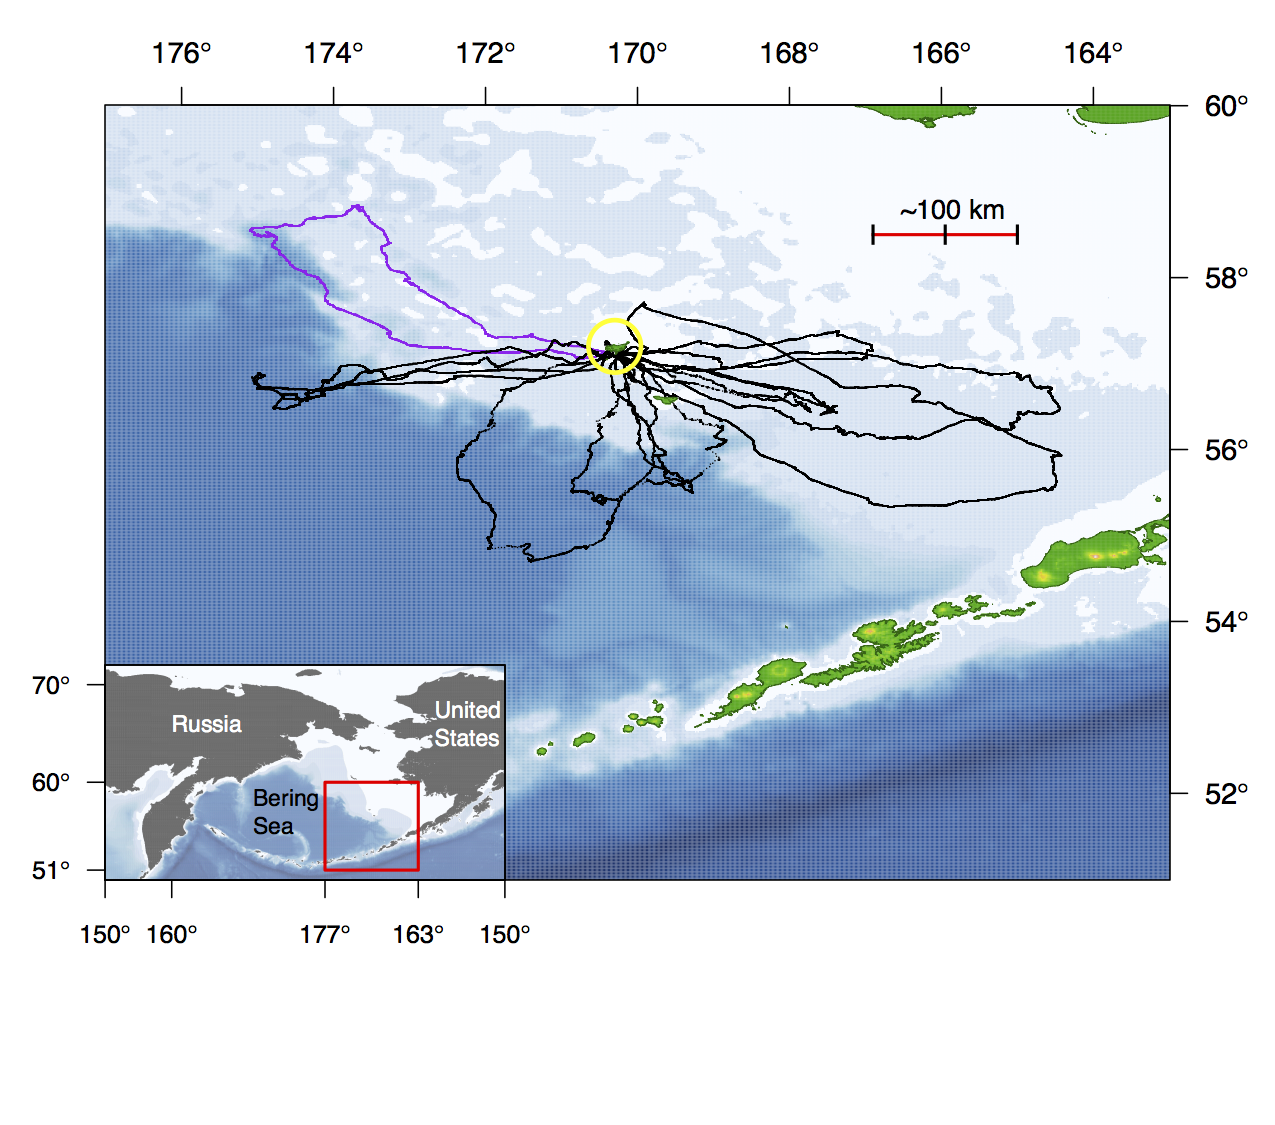
\includegraphics[width=7.25in]{fig1ugg.png}}
\caption{Eleven at-sea foraging tracks of lactating female northern fur seals tagged at Reef Rookery on St. Paul Island, in the Pribilof Islands in the Bering Sea, Alaska, USA.  St. Paul Island is circled in yellow. The seal represented in Figure \ref{f:recontrack} is coloured in purple for reference. Darker shades of blue indicate deeper ocean bathymetry, in particular the transition from light blue to dark found west of St. Paul Island indicates the location of the continental shelf break (also refer to Figure \ref{f:MAP2} in the introduction).} 
\label{f:MAP3}  
\end{figure} 


\subsection{Behaviour Data}
\label{s:BEHAVDATA}
Once the fine-scale locations were resolved for all fur seal tracks, we identified fur seal behaviour along segments of track using an augmented state space modelling approach, with the aim of linked the solution space to a set of biological and physical variables that describe the changing at-sea environment. %collated spatially, temporally linked external data. 

We identify the behavioural response variable by following the augmented state space methods described in Dowd and Joy (2011) on the archival dead-reckoner tag. Our analysis proceeds by differencing the tag's depth channel to create a measure of ``vertical velocity". The 2- or 5-second resolution data series of vertical velocity is then sectioned into 26 minute windows over which we use a discretized $2^\textrm{nd}$-order ordinary differential equation (AR-2 difference equation) as the process model in the augmented state space. The process model's continuous parameter solutions describe fur seal vertical movement and can be translated to classifications of behaviour by studying the qualitative form of the general solution to the AR-2 difference equation. We applied a locally optimized kernel smoother to the continuous parameter solutions to compensate for errors from unresolved tag measurement error and the random stochasticity in state space solutions (Herrmann 2003, R library ``$lokern$"). For each time window, we use the numerical properties of the parameter solutions to define the conditions for uncorrelated pseudo-periodicity, asymptotic stationarity and white noise (Priestly 2004, Shumway and Stoffer 2006), and relate these to three unordered discrete behaviour classes: ``Active Diving", ``Exploratory Diving", and ``Non-Diving" (Dowd and Joy 2011). 

For example, the solution space for the state space parameters describing movement identifies two distinct regions that characterize unique numerical properties (Figure~\ref{f:PHASEPLANE}). We interpret solutions that fall in the yellow region as repetitive diving reminiscent of an oscillating pendulum, and call this behaviour mode ``$Active$ $Diving$".  Parameter solutions that fall in the red area represent more intermittent diving characterized by a correlated random walk. We call the behaviour mode, ``$Exploratory$ $Diving$". 

\begin{figure}
\centerline{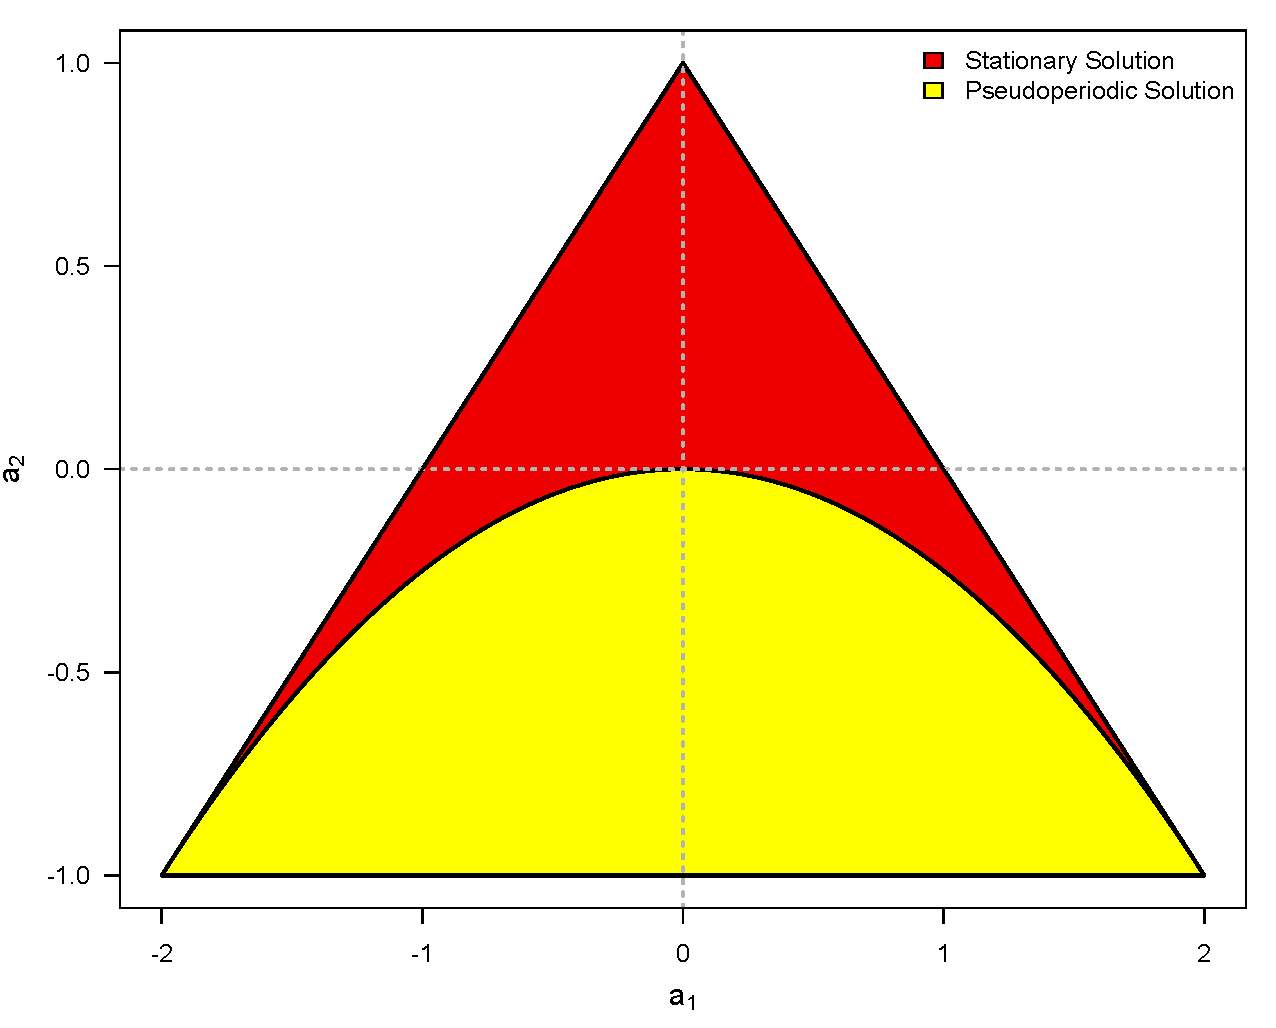
\includegraphics[width=7.25in]{phaseplane.pdf}}
\caption{Parameter plane for the solution space of a set of movement parameters $a_1$ and $a_2$ that solve a set of stationary AR(2) difference equations.} 
\label{f:PHASEPLANE}  
\end{figure} 

Vertical velocity is small for both sleeping or resting animals and for horizontal surface movement such as transiting, and hence we could not distinguish between these two modes. For purposes of the behavioural analyses, transiting, resting, and sleeping were considered the same non-diving behavioural state, as these behaviours are characterized by a lack of engagement in the immediate environment. We used the off-line estimate of system variance for each window for vertical speed (described in Appendix \ref{app:Appendix1} of Dowd and Joy 2011) to identify non-diving states (eg. Figure \ref{f:3March16}). We called this behaviour mode, ``$Non$-$Diving$".

For illustration, Figure (\ref{f:behavplot}) demonstrates the movement parameters and corresponding behaviour for Track 3 for a single day (August 18$^{\textrm{th}}$, 2006). Figure (\ref{f:D3Christina}) shows how the fine-scale 3-D movement for the entire track is translated into the three behaviour modes. \\


\begin{figure}
\centerline{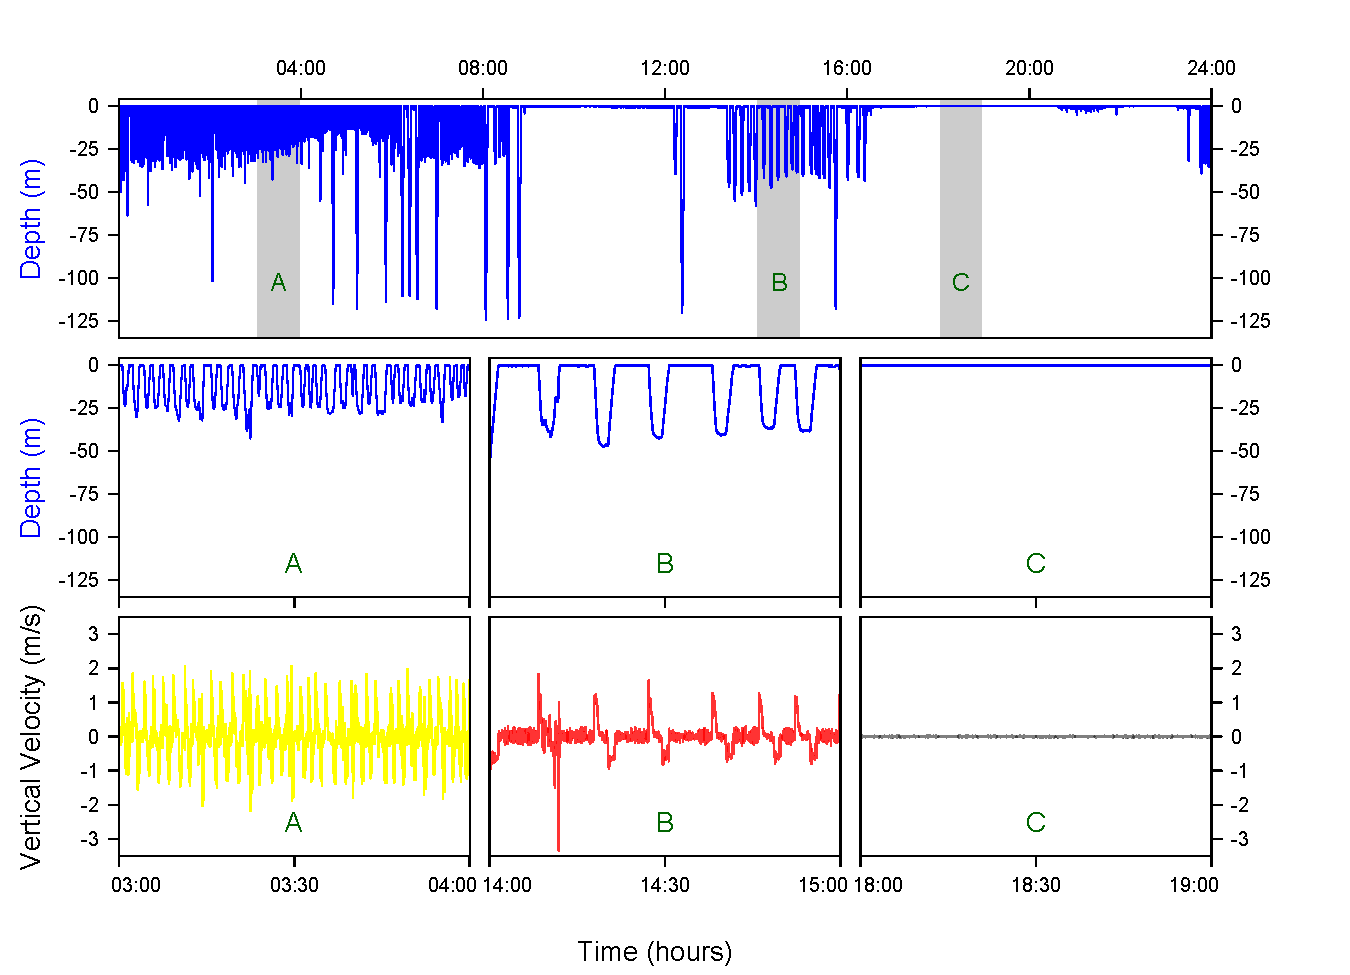
\includegraphics[width=16.1cm]{DEPSPEED.pdf}}
\caption{Observed time series taken from an archival tag for ``Track 3'' showing depth and derived vertical velocity of dives over a 24 hour period on August 18$^{\textrm{th}}$, 2006. Upper and middle panels show depth (in blue). The three lower figures shown in yellow, red and black, represent the  vertical speed variable derived from the depth channel. These lower panels highlights three 1-hour periods stretched out accordion-style to better see the features of this high density data series and show the three northern fur seal behaviours identified in our models. Region $A$ corresponds to a section of ``'$active$ $diving$"; Region $B$ corresponds to a section of ``$exploratory$ $diving$"; Region $C$ corresponds to an area of ``non-diving". This data section is linked to Figures (\ref{f:MDRJFIG1}), (\ref{f:MDRJFIG1b}), (\ref{f:3March16}) and (\ref{f:2March16}) in Chapter (\ref{s:twoA}).  }
\label{f:DEPSPEED}  
\end{figure} 

\begin{figure}
\centerline{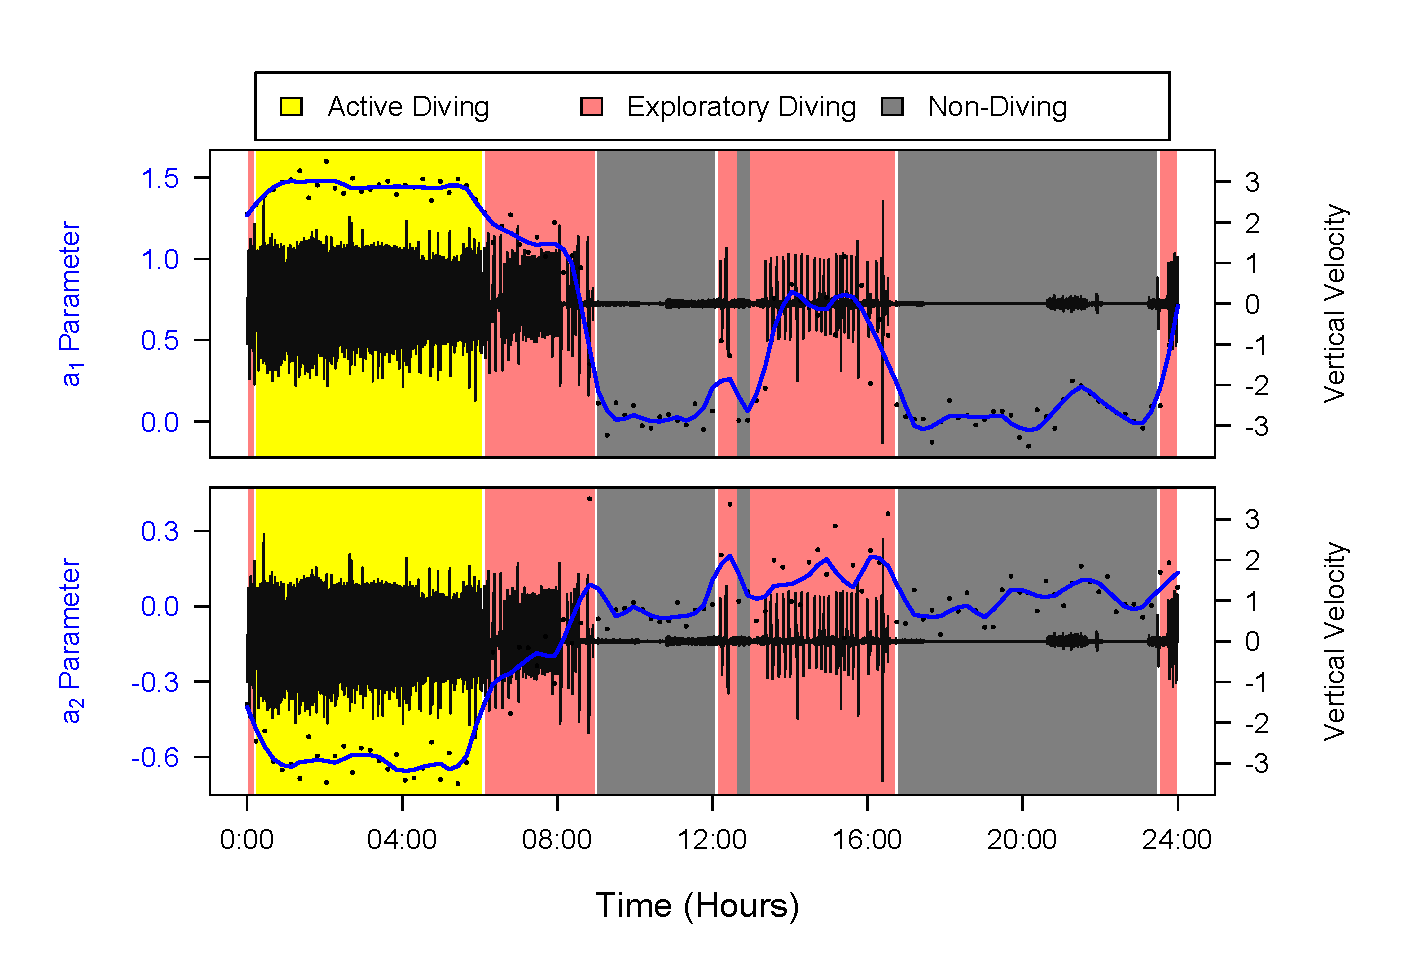
\includegraphics[width=16.1cm]{behavplot.pdf}}
\caption{Time series for Track 3 of the smoothed movement parameters (blue line) overlaid with the original data series of vertical velocity (black lines) for a single day. These coloured blocks correspond to regions in the parameter plane for the solution space of a set of AR-2 difference equations, and regions of minimal system noise variance. The block coloured $yellow$ corresponds to a region of ``'$active$ $diving$", the block coloured  $pink$ corresponds to an area of ``$exploratory$ $diving$", the block coloured  $grey$ corresponds to an area of ``non-diving". Recall Figure (\ref{f:PHASEPLANE}) depicting the phase plane. See also Figure \ref{f:3March16} for the associated plots of the series' system noise and observation error variances, and Figure (\ref{f:DEPSPEED}) for the original data series for this same day, August 18$^{\textrm{th}}$, 2006. }
\label{f:behavplot}  
\end{figure} 

\begin{figure} 
\centerline{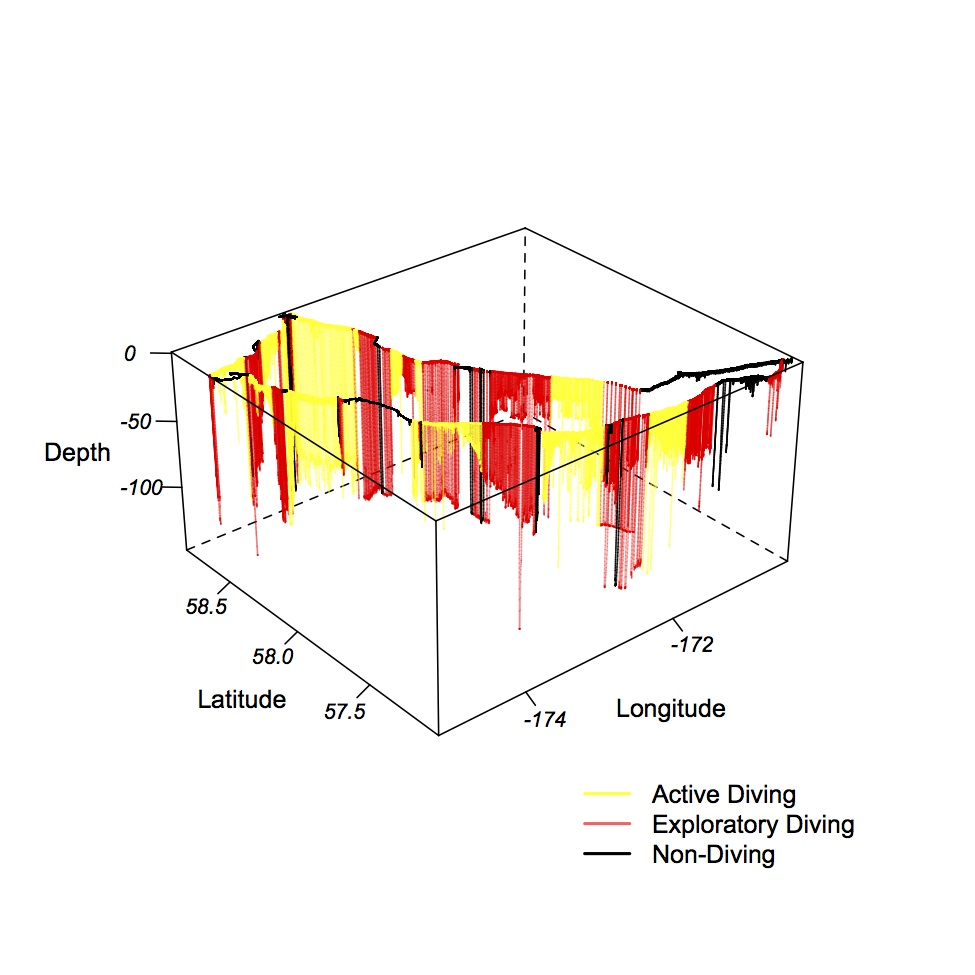
\includegraphics[trim=0 10 0 80,clip,width=17cm]{D3Christina.jpg}}
\caption{Three-dimensional reconstruction of a single northern fur seal's 11.2 day at-sea foraging track with assigned behaviour overlaid in space and time. This track corresponds to the same track (Track 3) pictured in Figures \ref{f:CorrSpeed} $-$ \ref{f:behavplot}. Reef Rookery (start/end point) is located at the far right of this figure, the fur seal swims closer to the viewer on the way out, and returns to the rookery farther from the viewer, by way of a long transiting section. } 
\label{f:D3Christina}  
\end{figure} 

We concatenated similar 26-minute windows of the behavioural types together into coherent ``segments" of similar behaviour. This better relates the observed seal behaviour to the scale of the spatial covariate information and defines the response variable as the observed behaviour of a fur seal over a variable-length segment of time and space. Each behaviour mode of each female fur seal is then associated in space and time to a position in the Bering Sea that changes as the fur seal moves. 



% ----- start of giant paste -----
\subsection{At-Sea Environmental Conditions: Covariate Data}
\label{s:DATA}

\subsubsection{Commercial Groundfish Catch and Walleye Pollock} 
A major goal of the study was to ascertain the extent (if any) to which fur seal behaviour was associated with fish abundance, and in particular, walleye pollock density. As a proxy for fish abundance we used the US Department of Commerce domestic observer data of the Alaska groundfish fishery for 2004-2008 (NMFS 2012).  We spatially linked the fur seal tracks to each groundfish haul to the nearest 1/60th of a degree longitude and latitude ($\sim$1.85 km). We selected 2 variables of interest; the first was total catch weight for each groundfish haul (including both retained and discarded species), and the second was haul weight of walleye pollock. 

We limited the fish catch data to July 9th, the beginning date of the breeding season (Trites 1992), and November 11th in 2005, and November 18th in 2006, the median dispersal dates for pups on St. Paul Island (Lea et al. 2009). 
Initially, we matched fishing effort by year to our track data but found the catch data for 2005 and 2006 were too sparse to be reliable. Therefore we included all data for the years 2004 through 2008, with the acknowledgment that although small scale commercial fishing hotspots change over years, by including multiple years we had smoothed over temporal variability, but captured persistent spatial hotspots. Where multiple hauls were linked per track segment, we took the median catch weight and median pollock weight to represent that segment of track.  

 for each of the behavior states along the length of each foraging track. Where multiple hauls were linked for a single segment of track, we took the median haul measurement for that behaviour segment as representative.

\subsubsection{Sea surface temperature}
Sea surface temperature data was retrieved from the dead-reckoner tag. We filtered all data that were observed outside of the top two metres of the ocean surface. 

\subsubsection{Primary Productivity}
We assigned primary productivity over the foraging track by constructing a composite field of weighted averages along the fur seal�s track by linearly interpolating time between the 8-day NOAA CoastWatch net primary productivity product\\ ($http://coastwatch.pfeg.noaa.gov/coastwatch/CWBrowserAK.jsp$) to match the time and location of the fur seal track. This derived measure of net primary productivity is based on satellite-collected chlorophyll-a concentration and photosynthetically available radiation (PAR) measurements, corrected for the amount of organic carbon used by planktonic organisms in respiration (Behrenfeld and Falkowski, 1997), and gridded at 1/6th of a degree ($\sim$18.5 km). This was done so that each female's track was overlayed with a slightly different productivity field that was linked to the particular time range and location of each foraging trip. 

\subsubsection{Wind Speed}  %-1.04719755
Also for each 24 hour period, we extracted NCDC blended satellite wind speeds at 17:00 local time (http://www.ncdc.noaa.gov/oa/rsad/air-sea/seawinds.html).  This wind speed product blends satellite wind speeds from multiple platforms such as scatterometers, and passive microwave radiometers (Zhang et al. 2006). The best nominal resolution is 1/4 degree (~28km) but as winds are spatially coherent on scales of hundreds of kilometres, we estimated wind speed once per day of each track, at the midpoint of the entire track and used linear interpolation across time to estimate windspeed for each behavioural segment. 

\subsubsection{Ocean Depth} 
As the bathymetry of this region of the Bering Sea is dominated by on-shelf shallow waters $<200$ metres deep and off-shelf waters with ocean depths of 3000 metres or more, we simplified bathymetry into an on-shelf/off-shelf categorical variable. Note the maximum dive depth of a northern fur seal is $\sim$200 metres (Gentry et al. 1986). For ocean depth data, we matched longitude and latitude of the track to the nearest depth measurement from the ETOPO1 bathymetry model \\($http://www.ngdc.noaa.gov/mgg/gdas/gd_designagrid.html$, Amante and Eakins 2009), which gives bathymetry output in arc minutes, 1/60$^{th}$ of a degree, ($\sim$1.85 kilometers). We then calculated the median depth for each of the behavior states along the at-sea track. For example if the seal was in an active diving mode between midnight and 4am, we took the median depth of the ocean during that period of the track, and classified it as on-shelf or off-shelf. We also followed methods and depth definitions of Call et al. (2008) and described depth as a three level categorical variable: inner/middle shelf (0-100 m), outer shelf (100-200 m), and off-shelf ($>$200 m). 

\subsubsection{Time of Day}
Time for each behavioural state was taken once from the dead-reckoner tag at the start of each behavioural period. As northern fur seals have strong circadian patterns in behavior (Ream et al. 2005), we transformed the time of day into a circular variable to capture this periodic rhythm, and to ensure that the interpretation of time at 24:00 is equal to that at 00:00. We modelled the dependence on time of day as a sine wave with a 24 hour period. %transformed hour of day using a trigonomic identity into a covariate vector of length two by taking the sine and the cosine of the hour expressed in radians for a 24 hour period. This ensures that the interpretation of time at 24:00 is equal to that at 00:00, and describes behaviour for one full 24 hour period as a sinusoidal function.  \\
% arctan2 function : to define the able between 2 points on a circle., where x is defined on a circle as a unit vector. 
Using a standard trigonometric identity, we rewrite $time$ $of$ $day$, $t$, as a sine wave with a 24-hour period as follows
\begin{eqnarray}
A \,\,sin \left(\frac{2 \pi t}{24} + \phi \right) &=& A \,\,sin(\phi)\,\, cos \left( \frac{2 \pi t}{24} \right) + A \,\, cos(\phi)\,\, sin \left( \frac{2 \pi t}{24} \right) \nonumber \\ \nonumber \\
&=& \alpha_1 \,\,cos \left(\frac{2 \pi t}{24} \right) + \alpha_2\,\, sin \left(\frac{2 \pi t}{24} \right) \,\,\,\, ,%\textrm{pg 67 Shumway et al.}
\label{eq:CIRCLE}
\end{eqnarray}
where $A$ is the amplitude of the wave, $\phi$ is the phase shift, $\alpha_1= A\,\, sin(\phi)$ and $\alpha_2= A \,\,sin(\phi)$. This provides a regression-type equation with the sine and cosine functions serving as the covariate data and $\alpha_1$ and $\alpha_2$ can be solved as regression parameters. %is the interpretation of the regression parameters $\alpha_1$ and $\alpha_2$ fit to the sinusoidal covariate function of time of day. 



\section{Methods}
\label{s:EMODEL}

Our goal was to see if the coupled environmental variables at each location could be used to provide insight into northern fur seal behavior. For this, we build the following hierarchical Bayesian model to examine the relationship between behaviour mode and at-sea habitat by matching the set of environmental variables in time and space to the observed behaviour model at the horizontal position of the fur seal's track. 

\subsection{Observation Model}
Our Bayesian hierarchical model begins with an observational process that describes fur seal behaviour and is accounted for via a likelihood or observation model. The multinomial probability density is one such observation model that relates the set of observed outcomes $\bm{y}$ to their outcome probabilities $\bm{p}$. Let $\bm{y}_{ij}$ be a random vector of length equal to the number of discrete behaviour outcomes or modes, where $\bm{y}_{ij}$ describes the behavioural response for the $i^{th}$ fur seal over the $j^{th}$ segment of track. The elements of $\bm{y}_{ij}$ are all zero except for the class of behaviour the fur seal is observed in, such that $\sum_{k=1}^Ky_{ij}^{(k)}=1$. 


\subsection{Local Process Model} \label{s:ProcMod}
The underlying (latent) probability vector describing the relative probabilities of each behaviour category  \{$p_{ij}^{(1)}, p_{ij}^{(2)}, \ldots , p_{ij}^{(K)}$\} can be linked to the set of covariates described in Section (\ref{s:DATA}), and a set of linear regression coefficients ($\bm{\beta}_i$), via a multinomial regression model for each fur seal (McCullagh and Nelder 1989). We model the logarithm of the ratio of the probability of each category relative to that of a baseline category, written logit $p_{ij}^{(k)}$, selecting the most commonly observed category, ``Non-Diving", as the denominator or baseline category, $p_{ij}^{(1)}$ , in the logit ratio (i.e. when $k=1$, baseline parameters $\bm{\beta}_i^{(1)}=0$), following the advice of Agresti (1990). 

The joint likelihood for the three categorical outcomes from the observation model and the multinomial process regression for all track segments for the $i^{th}$ fur seal can be rearranged and written

\begin{eqnarray}
\displaystyle
P (\bm{p}_i | \bm{X}_{i}, \bm{\beta}_i )   = exp   \left\{   \,\,\,
\sum_{k=2} ^{K} \left( \bm{\beta}_i^{(k)} \left[ \sum_{j=1}^{J_i} y_{ij}^{(k)} \bm{X}_{ij} \right] \right) - \sum_{j=1}^{J_i} {log} \left(1+\sum_{k=2}^K e^{\bm{X}_{ij}\bm{\beta}_i^{(k)}}\right) \,\,\,
     \right\}.  
     \label{eq:LIKELIHOOD2}
\end{eqnarray}

\subsubsection{Including Error in Covariates}
\label{s:EiCm}
An important aspect of process error problems is the difficulty in accurately estimating regression parameters when there is error contained within the covariate data (Stephens and Dellaportas 1992). Standard regression models assume that all covariates have been measured exactly, i.e. without error. In the case when some covariates are associated with error, estimation based on the standard assumption of no error in the covariates leads to biased and inaccurate inference about the true underlying covariate associations between regression covariates and response variable (Gustafson 2004).

In Equation (\ref{eq:LIKELIHOOD2}), all measured covariates for the $i^{th}$ fur seal were represented by $\bm{X}_i$. Henceforth, we distinguish between covariates measured with error, written as $\bm{W}_i$, and those without error, written as $\bm{Z}_i$. As well, we redefine $\bm{X}_i$ to be a covariate that we don't directly measure, but instead infer from observing the related variable $\bm{W}_i$. We are now assuming an implicit random effect model that is informed about the true data $\bm{X}_i$ through an error prone measure $\bm{W}_i$.  

The goal is to obtain unbiased estimates of regression parameters, $\bm{\beta}_{i}$ but the parameters of the regression of $logit \,\,\bm{p}_{i}^{(k)}$ on ($\bm{Z}_{i}, \bm{W}_{i}$) are different from those of $logit \,\,\bm{p}_{i}^{(k)}$ on ($\bm{Z}_{i}, \bm{X}_{i}$), and substituting $\bm{W}_{i}$ for $\bm{X}_{i}$, without adjusting the model for this substitution, leads to inaccurate and biased estimates (Gustafson 2004, Carroll et al. 2006). 

In our models, the major source of ``error" is due to the environmental field being divided up into behavioural segments, for which there is one measure per segment, and a single measure is likely an inadequate measure of the range of values experienced for that segment. If the observed covariate measure, $\bm{W}_{ij}$, is an index of a range of values over the $j^{th}$ segment of track for the $i^{th}$ fur seal, then we write an error model to reflect that the (latent) true measure, $\bm{X}_{ij}$, is more variable than its observed value, $\bm{W}_{ij}$ (Richardson and Gilks 1993, Carroll et al. 2006), and  form an error model as simple as  

\begin{eqnarray}
\bm{X}_{ij} = \bm{W}_{ij} + \bm{U}_{ij}.
\label{eq:MEASUREMENTMODEL}
\end{eqnarray}
We assume the observed covariate $\bm{W}_{ij}$ is unbiased for the true covariate $\bm{X}_{ij}$, and treat $\bm{W}_{ij}$ as fixed data in our Bayesian model thus allowing us to condition on it.  We assume $\bm{U}_{ij}$ is a normal, independent and identically distributed random variable according to $\sim \mathcal{N}(\bm{0}, \sigma^2_{iU})$ where $\sigma^2_{iU}$ describes the measurement error variance for the $i^{th}$ fur seal.  %, i.e. $E(\bm{U}_{ij} | \bm{W}_{ij}, \bm{Z}_{ij}) = \bm{0}$ and  $Var(\bm{U}_{ij} | \bm{W}_{ij}, \bm{Z}_{ij}) = \sigma_{iU}^2$.  
Measurement errors of the type found in Equation (\ref{eq:MEASUREMENTMODEL}) are called Berkson errors (Berkson 1950), and are typically chosen when all observations (along a segment of track) within an individual are given the same error-prone covariate. %

We treat the covariate model (Equation \ref{eq:MEASUREMENTMODEL}) as the prior for $\bm{X}_{i}$, selecting the multivariate normal distribution ($\mathcal{MVN}$) as the form of that prior, and select independent conjugate inverse gamma distributions ($\mathcal{IG}$) for $\sigma^2_{iU}$, i.e., 
\begin{eqnarray}
&& \bm{X}_{i} \sim \mathcal{MVN}(\bm{W}_i,{\sigma^2_{iU}} \mathcal{I}_{J_i}) \,\,\, \textrm{where $\mathcal{I}_{J_i}$ denotes an identity matrix of dimension $J_i$} \label{eq:P2}\\
&& \sigma^2_{iU} \sim \mathcal{IG}(a_U,b_{U}) \label{eq:P3} \,\,\,. %\textrm{ where $a_U=1$ and $b_{U}=3$.}
\end{eqnarray}
($cf.$ Appendix \ref{app:Conditionals} for justification of this and all following prior distributions). We used a Metropolis-Hastings step for sampling from the posterior distribution of $\bm{X}_i$, and used a Gibbs sampling step for sampling from the posterior of $\sigma^2_{iU}$. We selected $\mathcal{IG}({a_U}=3, {b_U}=1)$ as the prior distribution for $\sigma^2_{iU}$, but limited the sampling range for the prior to be within a factor of 5 standard deviations of the prior distribution mean. 

The following environmental covariates were modelled with error (1) total catch weight of groundfish haul, (2) haul weight of walleye pollock, (3) primary productivity, (4) sea surface temperature, and (5) wind. (Total catch weight and haul weight of walleye pollock were positively correlated ($r=0.85$), and therefore were not entered into the same model to protect analyses from matrix singularities.) We also considered (6) bathymetry (or on-shelf/off-shelf) and (7) time of day which were covariates that we assumed to be measured without error. We discuss the Bayesian priors for the lower level regression parameters, $\bm{\beta}_i$, in the following section. 

%%%%%%%%%%%%%%%%%%%%%%%%%%%%%%%%%%%%%%%%%%%%%%%%%%%%%%
\subsection{Population Parameter Model}
 %The lower-level specification of the model is specific to the individual animal, and expresses the uncertainty we have about that animal's response to the ecological process we would like to understand.  
The population model links the lower-level models for each fur seal. This is done by selecting a joint prior for the lower-level regression parameters, $\bm{\beta}$, as the population model.  It is natural to give the parameters of all 11 fur seals a common distribution, and develop this level of hierarchy that has the advantage of providing a single unified probability framework. We selected the multivariate normal distribution as a joint prior of the lower-level regression parameters:
\begin{eqnarray}
&& \bm{\beta} \sim \mathcal{MVN}(\bm{1}\bm{B},\bm{\Sigma}_{\beta}) \label{eq:P1}.
\end{eqnarray}
This shared prior distribution for $\bm{\beta}$ that links all the lower-level models and forms a higher-level multivariate normal likelihood as the population model. 
The following inverse Wishart ($\mathcal{IW}$) and multivariate normal distributions were selected as hyper-prior distribution for the variance and mean of the prior for $\bm{\beta}$, i.e.,
\begin{eqnarray}
&& \bm{\Sigma}_{\beta} \sim \mathcal{IW}(\nu_0,\bm{V}_0) \label{eq:P4}\\
&& \bm{B}| \bm{\Sigma}_{\beta} \sim \mathcal{MVN}(\bm{B}_0, \frac{1}{a_0}\bm{\Sigma}_{\beta}) \label{eq:P5}.
\end{eqnarray}
We chose a diffuse inverse Wishart prior distribution that had parameters $\nu_0=m+3$ degrees of freedom (such that $\nu_0>m$), and scale matrix $\bm{V}_0=\nu_0 \times \mathcal{I}_m$ where $\mathcal{I}_m$ denotes an identity matrix of dimension m; i.e. $\Sigma_{\beta}$ and $\mathcal{I}$ are $m$ by $m$ matrices. We selected the multivariate normal distribution with mean $\bm{B}_0=\bm{0}$, a vector of zeros of length $m$, and variance $\frac{1}{a_0} {\bm{\Sigma}_{\beta}}$, where $a_0=0.01$ to make the scale matrix diffuse. 
As the priors for both $\bm{B}$ and $\bm{\Sigma}_{\beta}$ were conjugate to the higher-level $\mathcal{MVN}$ likelihood, we sampled from these posteriors using a Gibbs sampling step. 

By linking regression models via a shared prior, we acknowledge a different source of randomness, the variability in the population (Cressie et al. 2009) and can ``borrow strength" between animals (Ntzoufras 2009). We can now think of the set of regression parameters specific to a single animal (e.g. $\bm{\beta}_i$) as a sample from a distribution of possible values (i.e. random coefficients), and the posterior of each unit-level $\bm{\beta}_i$ is then a weighted mean of the corresponding animal's regression and the overall population effect.  

%%%%%%%%%%%%%%%%%%%%%%%%%%%%%%%%%%%%%%%%%%%%%%%%%%%%%%%%%%%
\subsection{MCMC Model Set-up}
\label{s:ErrorMODEL}

We have described the set up of a hierarchical multinomial Bayesian error-in-covariate model to describe the relationship between a fur seal's behaviour and her environment, as described by matched covariates along a set of at-sea foraging tracks. By considering segments of track in which behaviour was consistent, and by matching each segment of track to one observation for each covariate, we have averaged over both temporal and spatial autocorrelation, and the analysis is somewhat simplified. We use a hierarchical framework that includes a lower-level parameter model for each tagged northern fur seal and describes the uncertainty in the relationship between each fur seal's behaviour and her at-sea environment, and then build a higher-level population model that describes the variability in the underlying process by assuming the set of tagged northern fur seals are a random sample from a population of similar animals nursing pups at Reef Rookery on St Paul Island in the Pribilof Islands. (Cressie et al. 2009). We implement an MCMC Metropolis-within-Gibbs sampling algorithm to sample from the joint state space of the model unknowns. 

We ran the MCMC simulation for 1,000,000 iterations. We used the partial correlation coefficient to fix the decimation rate for the MCMC chain. We fit autoregressive models of successively higher-orders until the lag suggested non-significant partial correlations between chain components. Chains were thinned to every $50^{\textrm{th}}$ iteration. 
We initialised the chains from three different starting points using different random seeds, but found posterior summary statistics were insensitive to initial conditions. 

We visually assessed convergence by inspection of MCMC trace plots, as well, we  calculated the Gelman-Rubin ($\hat{R}$) as modified by Brooks and Gelman (1998; using R library ``$coda$") as a quantitative measure of convergence. 


\subsection{Model Comparison and Model adequacy}
\label{s:GOF} 
\subsubsection {Information-Theoretic Model Selection}
Model comparison and selection is central to the scientific process by allowing different hypotheses to be evaluated about potential associations between variables (Pitt and Myung 2002). The best model from an $a$ $priori$ set of models and can be described as the one that explains the maximum level of detail in the simplest possible way (Burnham and Anderson 2002).  $AIC$ (Akaike 1973) estimates the relative information content of the models by trading off between the fit of the data to the model and the corresponding complexity of the model, and can be used in comparisons between non-nested models (Burnham and Anderson 2002). In hierarchical modelling, we cannot uniquely define a `likelihood' or `model complexity' without specifying the level of the hierarchy that is the focus of the modelling exercise (Gelfand and Trevisani 2002), i.e. inference at the population or at the individual level. Since we were interested in understanding fur seal behaviour in general and not simply the behaviour  (or prediction of the behaviour) of the sampled fur seals, inference around population parameters is the focus and marginal-likelihood methods such as $AIC$ are appropriate.

We report the posterior mean deviance $\overline{D(\Theta)}$ as a Bayesian measure of fit or ``adequacy" (Dempster 1974, Spiegelhalter et al. 2002),  $m_{DIC}$ as a diagnostic of leverage (Speigelhalter et al. 2002), as well as $AIC$. These provide useful comparisons between candidate models, but do not provide insight into model adequacy. 

\subsubsection{Model Adequacy: Goodness of Fit and Posterior Predictive Checks} %: $p_{pp}, R^B$ Comparing a model with and without error in covariates: 

We examined model adequacy through a series of distributional summaries. We compared posterior predictive distributions of replicated data under the model with the observed data (Rubin 1984; Gelman et al. 2004 p.175). If the model accurately represents the process that generated the data, then replicated data generated under the model should look similar to the observed data (Brooks and Gelman 1998).  An evaluation of closeness can be carried out using some summary function of discrepancy, $d(\bm{y},\bm{\Theta})$, with assessment of the overall goodness of fit using posterior predictive $p$-values (Meng 1994, Carlin and Louis 2000). The proportion of times the summary function of discrepancy, $d(\bm{y}_{rep}, \bm{\Theta})$, is less or equal to $d(\bm{y}, \bm{\Theta})$ is then recorded across iterations of the MCMC sampler, and used as a test of the model's capacity to reproduce the observed data. 

Due to uncertain large sample properties of posterior predictive $p$-values (for example, see discussion in Bayarri and Berger 2000), we assume that a $p$-value around 0.5 indicates that the distributions of the replicated and actual data are close, while a value close to zero or one indicates strong differences between them (Gelman et al. 2004). 

\subsection{Simulation to investigate implications of sample size}
\label{s:KL}
We constructed a simulation study using the Kullback-Leibler ($KL$) divergence statistic to examine the effect of sample size on model inference. The $KL$ divergence has been widely studied in statistical literature as a central index measuring qualitative similarity, or relative entropy, between two probability distributions, and is popular because it uses a likelihood ratio approach (Lee and Park 2006). We took 200 samples from the posterior distribution of the population-level models to use in generating 200 replicate datasets from each sample's posterior prediction. We then refit each of the 200 datasets using the MCMC model from which the data were generated. Posteriors of these replicate simulated datasets were gathered after burn-in, from a 10,000 long chain thinned to every 5$^{th}$ iteration. The $KL$ divergence for each of the original model's 12 population parameter posteriors $\bm{B}$ and the 200 simulated datasets and each of these model's parameter's posteriors were then calculated using R library ``$FlexMix$" (Leisch 2004).  




\section{Results}
\label{s:RESULTS}

\hilight{The results have to be made to correspond tightly to the methods} 

\hilight{It is good to refer back where possible explicitly  }


Ten of the eighteen lactating females captured at Reef Rookery yielded complete data sets from which the foraging paths and behaviour information could be retrieved. One of these animals provided data from two complete foraging trips giving us 11 complete foraging tracks. The remaining eight animals had only partial data records with lost data due to a number of tag failures including water entering the housing, the speed paddle breaking off, fish vertebrae lodged between the speed paddle and housing, and battery failure. We present the results of the behaviour analysis of the 11 complete northern fur seal foraging tracks from Reef Rookery on St. Paul Island during the pupping seasons of 2005 and 2006. Foraging trips ranged in length from 5.5 days to 11.2 days, with a median of 7 days spent at sea. There were an average of 40 ARGOS fixes, and 404,400 archival data records per trip. 

\begin{table}
\caption{\small{Summary of archival (data-logger) and Argos GPS tag data collected during 11 northern fur seal at-sea foraging tracks through the Bering Sea. Fur seals were tagged at Reef Rookery on St. Paul Island during the pupping seasons of 2005, 2006. The female corresponding to Track 3 who's track (or portions thereof) is visualised in Figures \ref{f:CorrSpeed}, \ref{f:recontrack}, \ref{f:MAP3}, \ref{f:behavplot}, and \ref{f:D3Christina} appears in \textbf{bold} font in this table. Tracks 5.1 and 5.2 correspond to the same female that took 2 trips and the tag was not recovered after her first at-sea track. Tracks 10.1, 10.2 correspond to the same tag that was deployed twice, on two separate and independent female northern fur seals. }
} 
\small
\bigskip
\begin{tabular}{l | rrrrrrrrrrr} 
\toprule 
\noalign{\smallskip}
   &\multicolumn{10}{c}{Female fur seal track ID} & \\
Variable & 1 & 2 & \bf{3} & 4 & 5.1 & 5.2 & 6 & 7 & 8 &10.1 & 10.2  \\
\midrule   \noalign{\smallskip}
\multirow{2}{*}{ Departure date} & Jul 13 & Jul 15  & \bf{Aug 16} & Aug 14  & Aug 13 & Aug 23 & Aug 13 & Aug 29 & Jul 16 & Aug 17 & Aug 26   \\
 & 2005 & 2005  & \bf{2006} & 2006 & 2006 & 2006 & 2006 & 2006 & 2005 & 2006 & 2006  \\
 &   &  & & & & & & & & &  \\
 Departure time & 23:31 & 02:15 & \bf{23:28} & 18:39 & 14:16 & 15:21&14:41 &07:23 & 01:14& 15:04& 11:46   \\
&   &  & & & & & & & & &  \\
 Return time  &  12:52 & 19:49 & \bf{03:52} &04:55 & 01:49& 17:09& 21:34& 04:11& 13:12& 15:29& 20:42  \\
&   &  & & & & & & & &  \\
 Trip length & \multirow{2}{*}{5.6}  & \multirow{2}{*}{6.7} & \multirow{2}{*}{\bf{11.2}} &\multirow{2}{*}{10.4} &\multirow{2}{*}{8.5} &\multirow{2}{*}{9.1} &\multirow{2}{*}{10.3} &\multirow{2}{*}{5.9} &\multirow{2}{*}{5.5} &\multirow{2}{*}{7.0} &\multirow{2}{*}{6.4}  \\
(days) &   &  & & & & & & & & &  \\
&   &  & & & & & & & & &  \\
    \# of Argos fixes    & 60 & 15  & \bf{74}  & 53  & 27  & 28  & 54  & 23  & 31 & 47 & 40  \\
&   &  & & & & & & & & &   \\
    \# of Argos GPS &  \multirow{2}{*}{10.7} &  \multirow{2}{*}{2.2}  &  \multirow{2}{*}{\bf{6.6}} &  \multirow{2}{*}{5.1}  &  \multirow{2}{*}{3.2 } &  \multirow{2}{*}{3.1}  &  \multirow{2}{*}{5.2}  &  \multirow{2}{*}{3.9}  &  \multirow{2}{*}{5.6} &  \multirow{2}{*}{6.7} &  \multirow{2}{*}{6.3}  \\
fixes per day & & & & & & & & & & &  \\
&   &  & & & & & & & & &  \\
 \# of archival&  \multirow{2}{*}{98800} & \multirow{2}{*}{291200} & \multirow{2}{*}{\bf{482400}} & \multirow{2}{*}{451600} & \multirow{2}{*}{404400} & \multirow{2}{*}{430400} &\multirow{2}{*}{445200} &\multirow{2}{*}{240000} &\multirow{2}{*}{94560} &\multirow{2}{*}{303200} & \multirow{2}{*}{406400} \\
tag data records     &   &  & & & & & & & & &  \\
&   &  & & & & & & & & &  \\
Sampling rate & \multirow{2}{*}{20} & \multirow{2}{*}{30}  & \multirow{2}{*}{\bf{30}}  & \multirow{2}{*}{30}  & \multirow{2}{*}{30}  & \multirow{2}{*}{30}  & \multirow{2}{*}{30}  & \multirow{2}{*}{30}  & \multirow{2}{*}{20} & \multirow{2}{*}{30} & \multirow{2}{*}{30} \\
per minute  &   &  & & & & & & & & & \\
\bottomrule
\end{tabular}
\label{tab:ONE}  
\end{table}


Figure (\ref{f:MAP3}) depicts the foraging track reconstructions highlighting the locations of these 11 foraging tracks in the Bering Sea. The fur seals traveled an average maximum linear distance from St. Paul Island of 279 km, with a maximum distance away of 391 km. Five animals stayed on the continental shelf, one animal moved along the shelf break foraging in the canyons, and 5 animals went across the shelf break into the deep water of the central Bering Sea. The one animal for which we had 2 successive trips (Tracks 5.1, 5.2) went to a similarly located feeding area off-shelf in both foraging trips. In general, these fur seals covered a wide area of both on-shelf and deep, off-shelf waters in the Bering Sea and showed no preference for foraging in any single area. 

Fur seals spent 35\% of the time at sea engaged in either active (14\%) or exploratory dives (21\%). Fur seals spent 65\% of time at the surface engaged in non-diving behaviours. The 11 foraging trips had a median of 41 segments in different behaviour modes, with those animals with longer foraging trips exhibiting more behaviour changes.  Figure (\ref{f:behavlen}) plots the distribution of segment lengths of track. This figure shows that for all 421 behaviour segments observed across all animals, the most commonly observed segment length was $<1$ hour, but this was by far the most frequent time length for active diving segments (44\%), whereas exploratory diving and non-diving segments were comparatively less likely to be $<1$ hour (26.5\% and 15.1\% respectively).

A three-dimensional reconstruction of one at-sea foraging route (Track 3) is presented in Figure (\ref{f:D3Christina}) in which behaviours are identified by changes in colour.


\begin{figure}
\centerline{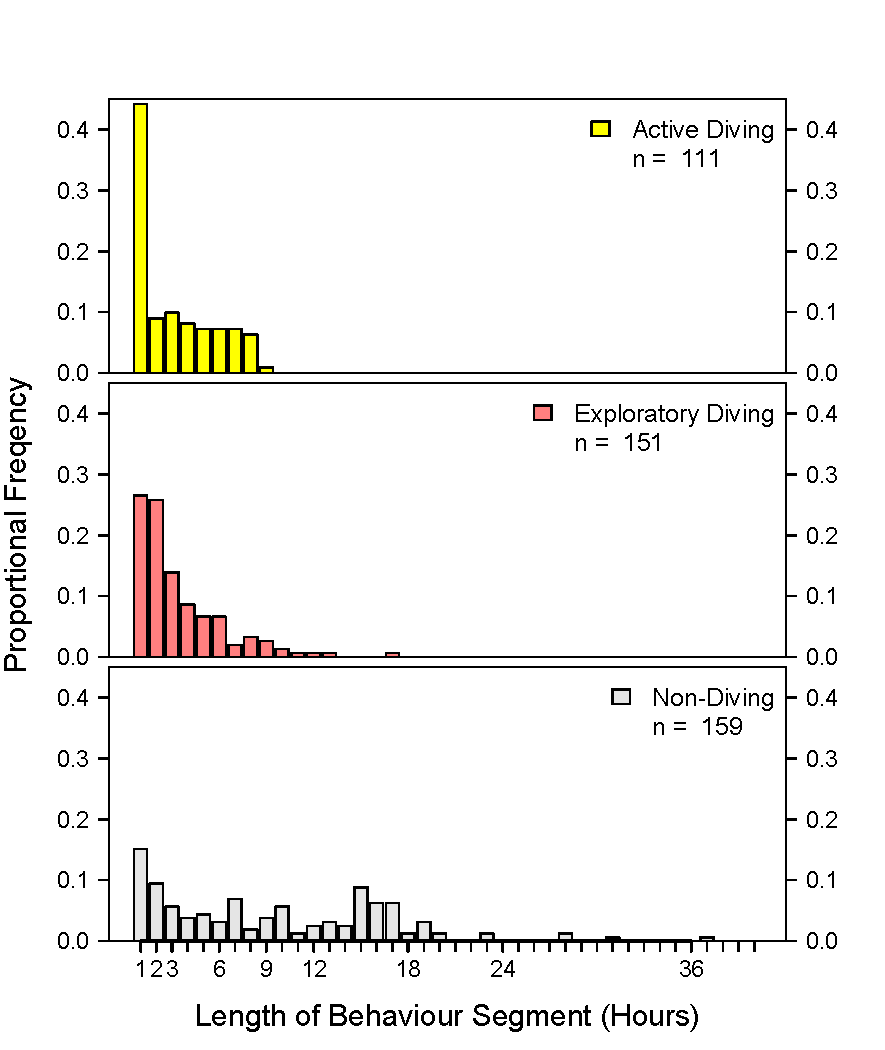
\includegraphics[trim=0 -10 0 0, clip, width=14cm]{behavlen.pdf}}
\caption{Length distribution of 421 behavioural segments measured from 11 at-sea foraging tracks of female northern fur seals. Each panel shows the distribution of one of the three behaviour states: $active$ $diving$, $exploratory$ $diving$ and $non$-$diving$, where each bar represents the relative frequency of observed segments of lengths up to that hourly measure. For example, the first bar labeled ``1" represents the frequency distribution of segments between 0 and 1 hour long, the second bar labeled ``2" represents the frequency distribution of segments between 1 and 2 hours long, $etc$. }
\label{f:behavlen}  
\end{figure} 

\begin{figure} 
\centerline{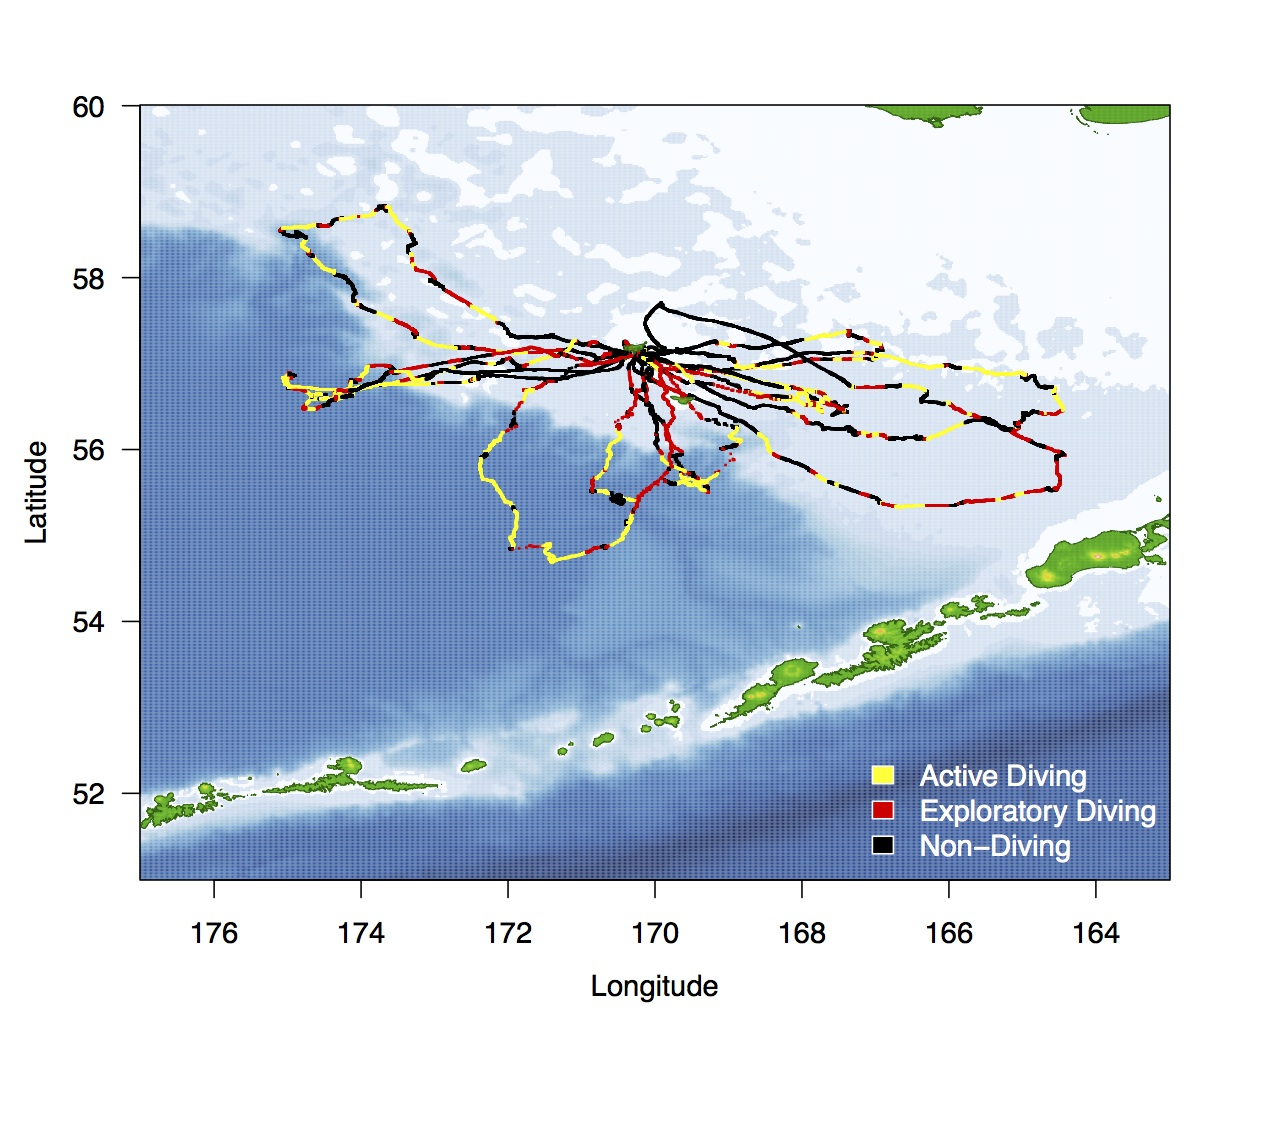
\includegraphics[width=15cm]{fig4perhaps.jpg}}
\caption{Identified behaviours of northern fur seal overlaid on eleven at-sea foraging tracks of lactating female northern fur seals from St. Paul Island, Alaska. }%(we also refer reader to Figure \ref{f:MAP2} and  \ref{f:MAP3}). ALSO... can you mark which traces are which with labels -- 1:10.2
\label{f:MAP4}  
\end{figure} 

\subsection{Model selection}
We fit all main effect models with covariates described in Section (\ref{s:DATA}). The strongest univariate predictor of behaviour was time of day ($Time$; Table \ref{t:TWO}), but behaviour was also found to be related to total (logged) haul size of all catch ($Total\,Catch$) and (logged) haul weight of walleye pollock ($Pollock$). We found behaviour unrelated to bathymetry, primary productivity,  sea surface temperature or wind. 

We then fit a series of models that all included time of day ($Time$) and one by one (additive) inclusion of the remaining covariates. Models fit with $Pollock$ and $Total\,Catch$ and bathymetry (\textit{On/Off Shelf}) were the best subset by the model selection criteria presented earlier. $Total\,Catch$ was related to behaviour (significant Bayesian $p$-value), but bathymetry was unrelated (Table \ref{t:TWO}). We found that the three depth categories described by Call et al. (2008) were not an improvement over the simplified depth categories (on $vs.$ off-shelf) and are not discussed further. 

We next fit a set of models with $Time$, another main effect, and a $Time \times main\,$\textit{effect} interaction. The two models with time interacting with a measure of groundfish catch had the best fit diagnostics ($Pollock$, $Total\,Catch$; Table \ref{t:TWO}). 

The model that included time of day and primary productivity failed the posterior predictive test, suggesting the model didn't fit the data well, despite having adequate higher-order parameter convergence in their respective MCMC's (i.e. $\hat{R} \approx 1$). We failed to get satisfactory convergence ($\hat{R} \gg 1$) with covariates sea surface temperature and wind, and these results are omitted from Table (\ref{t:TWO}). 

One additional step of model complexity was considered. We fit a three covariate model based on the best time-interaction model, and bathymetry (Time $\times$ Pollock $+$ \textit{On/Off Shelf}). This model was penalized aggressively, suggesting the additional complexity was not warranted despite a fair goodness of fit to the data. Table (\ref{t:TWO}) reports a subset of the results from the model fitting. 

 \begin{table}
\caption{Model information criteria, and model fit diagnostics. $AIC$ is a relative measures of model fit (smaller implies better fit), $\overline{D(\bm{\beta})}$ is a measure of model adequacy (smaller implies better fit), $m$ represents the number of population parameters in the upper level model, and $m_{DIC}$ is an estimate of effective number of model parameters. Posterior predictive $p$-values ($p_{pp}) > 0.05$ implies there is no evidence model is predicting poorly. 
}

 \vspace{5pt}
    \begin{tabular}{l | c | c | c | c | c  }    
    \toprule   \noalign{\smallskip} 
      & ~~ & ~ &~ & ~ & ~   \\ 
  Model Name   & $AIC$ &  $\overline{D(\bm{\beta})}$ &  m & $m_{DIC}$ &  $p_{pp}$ \\ \hline
       &  ~ & ~ & ~ & ~  &  \\
Time Only                   & 346.5 &  351.3 & 6 & 31.9 &  0.80 \\ % time.only.model
       \bottomrule
   \toprule   \noalign{\smallskip} 
      Time  and Main Effect & ~ &~ & ~& ~ & ~    \\  
     Models & $AIC$ & $\overline{D(\bm{\beta})}$ &  $m$ &  $m_{DIC}$ & $p_{pp}$   \\ \hline
            &  ~ & ~ & ~ & ~  & ~  \\
       Time + Total Catch & 290.1 & 349.9 & 8 & 38.9  & 0.55  \\  % main.catch
       Time + Pollock & 290.0 &  344.0   & 8 &  37.8 &  0.72 \\  % main.poll
       Time + On/Off Shelf & 298.7 & 344.5 &  8  & 40.8 &  0.84  \\  % main.bath1 NO ERROR as it's categorical
       Time + $1^{\circ}$ Productivity & 382.0 &  344.0 &  8 & 40.2 &  0.04 \\  % wind.rhierMnlRwMixture.100002
       \bottomrule
   \toprule   \noalign{\smallskip} 
      Time  Interaction  & ~ &~ & ~& ~ & ~    \\  
     Models & $AIC$ &  $\overline{D(\bm{\beta})}$ &  $m$  &  $m_{DIC}$ & $p_{pp}$ \\ \hline
       &  ~ & ~ & ~ & ~  & ~   \\
  Time $\times$ Total Catch & 285.6 & 322.8 &  12 &  48.5  & 0.32  \\ % junk5-8
\textbf{Time $\times$ Pollock}        &  \bf{284.3} &  \bf{323.2} & 12 & \bf{44.3} &  \bf{0.72}  \\ % poll.model
      Time $\times$ On/Off Shelf      & 303.6  & 330.8 & 12 & 51.8  & 0.62 \\ % bath1.model in units like Call et al.
      Time $\times$ $1^{\circ}$ Productivity    & 292.0 &  334.7 &  12 & 60.0  & 0.00 \\ % primp.model
         \bottomrule
   \toprule   \noalign{\smallskip} 
      Three Covariate  & ~ &~ & ~& ~ & ~   \\  
     Model & $AIC$ &  $\overline{D(\bm{\beta})}$ & $m$ &   $m_{DIC}$ & $p_{pp}$ \\ \hline
       &  ~ & ~ & ~ & ~  & ~   \\
      Time $\times$ Pollock + On/Off Shelf &  332.3 &  314.1 & 14 &   66.2  &  0.51  \\ % poll.model
       \bottomrule
 \end{tabular}
\label{t:TWO}  
\end{table}

We considered a small subset of models for comparison of model fit with and without including measurement error in the covariates. In Table (\ref{t:THREE}) and Figure (\ref{f:CI95}), we see that the effect of including the measurement error in the model is to shrink the regression parameters towards zero, and to increase the uncertainty around the estimates of those parameters. Table (\ref{t:THREE}) compares the model fit diagnostics, information criteria and posterior predictive checks both with and without error-in-covariates. By including the uncertainty in the measurement of haul size of pollock, the model fits significantly better. 


\begin{table}
\caption{Comparing a selected model with and without consideration of the error in model covariates. This table presents model fit diagnostics for which the descriptions and definitions are comparable to those in Table (\ref{t:TWO}).}
%} 
\vspace{5pt}
    \begin{tabular}{l | c | c | c | c | c }    
    \toprule   \noalign{\smallskip} 
     Time $\times$ Pollock & ~ & ~ & ~ & ~   \\  
     Models & $AIC$  & $\overline{D(\bm{\beta})}$ & $m$ &   $m_{DIC}$ & $p_{pp}$   \\ \hline
       &  ~ & ~ & ~ & ~  & ~  \\
      Time $\times$ Pollock without $\bm{\sigma^2}_U$ & 297.0  & 329.4 & 12 &  58.8  & 0.461  \\ % junk4
\textbf{Time $\times$ Pollock with $\bm{\sigma^2}_U$} &  \bf{284.3}  & \bf{323.2} & \bf{12}& \bf{44.3} &  \bf{0.72} \\ % junk5-8
\bottomrule
\end{tabular}
\label{t:THREE}  
\end{table}

Our final selected model (Time $\times$ Pollock with error in covariates) suggests that female at-sea behavior was influenced by time of day, and (logged) haul size of walleye pollock. $Time \times Total\,Catch$ was a similarly good model with only marginally poorer criteria based on $AIC$, with similar model adequacy measures ($\overline{D(\bm{\beta})}$), but a larger number of parameters estimated as implied by comparison of $m_{DIC}$. Coefficient magnitudes, and signs were similar for both models. Figure (\ref{f:CI95}) and Table (\ref{t:bees}) depict the 95\% credible intervals for each of the population parameters, and shows significance for the main effect of time of day, and for the interaction of time of day and haul size of pollock.

\begin{figure} 
\centerline{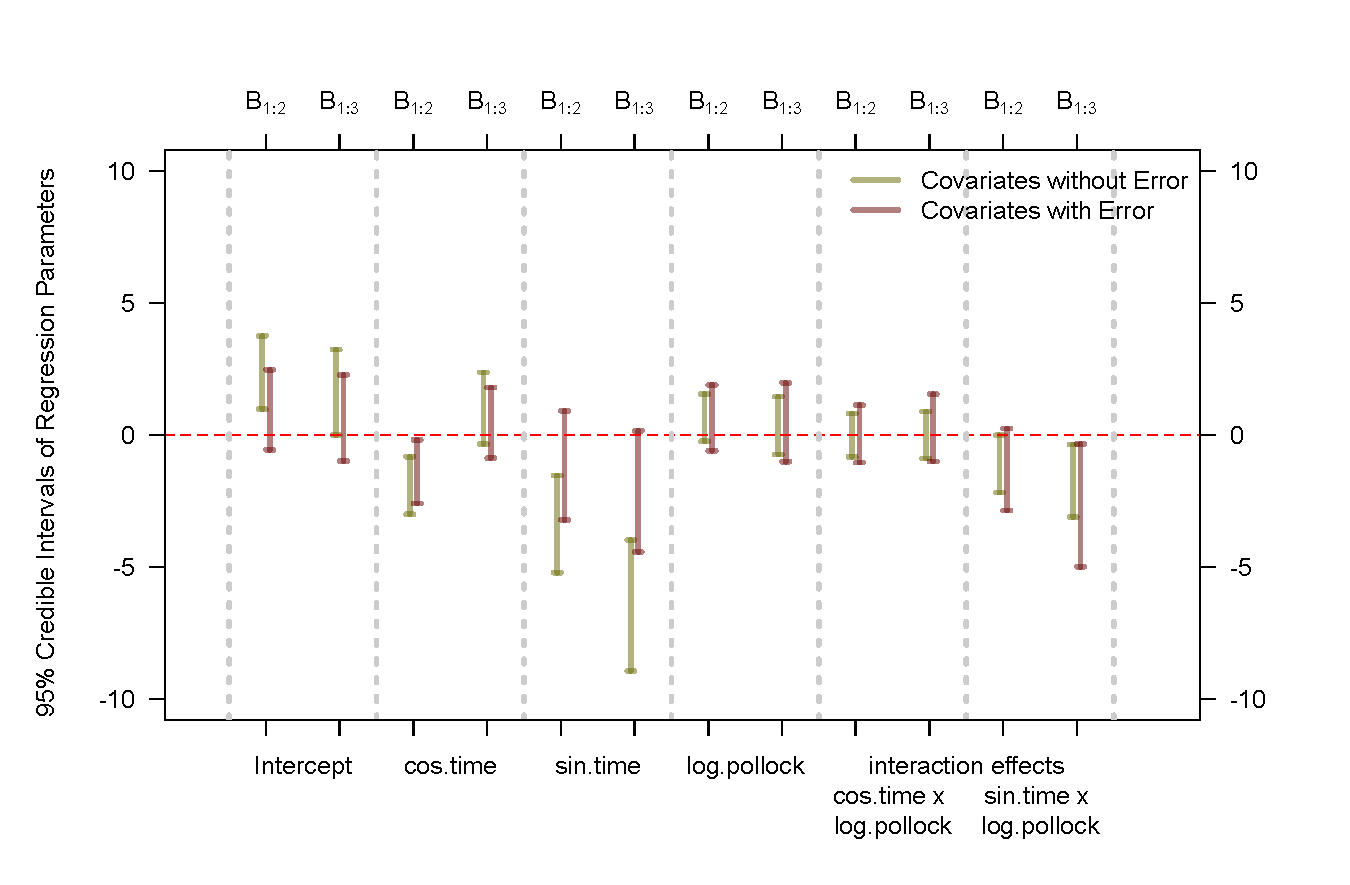
\includegraphics[width=16.5cm]{CI95.pdf}}
\caption{95\% credible intervals for twelve regression parameters ${\bm{B}}$ from the population level model that includes $time$ $of$ $day$ and (logged) haul size of $pollock$ (Time $\times$ Pollock) measured without error and with error. Each pair of ${\bm{B}}$ coefficients show the credible intervals of the population-level parameters linking northern fur seal behaviour to at-sea habitat. $B_{1:2}$ denotes the regression parameters corresponding to the logit response $log (p_{ij}^{(2)}/p_{ij}^{(1)} )$, or the log odds of exploratory diving vs. baseline non-diving. $B_{1:3}$  denotes the regression parameters corresponding to the logit response $log (p_{ij}^{(3)}/p_{ij}^{(1)} )$, or log odds of active diving vs. baseline non-diving).}
\label{f:CI95}  
\end{figure} 

%---------------\clearpage
\begin{table}
    \centering
\caption{Posterior summaries for higher level model coefficients $\bm{B}$. $B_{1:2}$ denotes the regression parameters corresponding to the logit response $log (p_{ij}^{(2)}/p_{ij}^{(1)} )$, or the log odds of exploratory diving vs. baseline non-diving. $B_{1:3}$  denotes the regression parameters corresponding to the logit response $log (p_{ij}^{(3)}/p_{ij}^{(1)} )$, or log odds of active diving vs. baseline non-diving). The column labeled $\hat{R}$ is the Gelman-Rubin Bayesian measure of convergence. Parameters with significant Bayesian $p$-values are noted in $\bm{bold}$.  }
%\rowcolors{1}{white}{gray}
    \begin{tabular}{ll | rr | rrrr  }    
     \hline   \noalign{\smallskip} \hline
       & ~ & ~ & ~ & Median  & \multicolumn{2}{c}{Credible Interval} & ~\\  
      & ~ & Mean & St. Dev. & $q_{.5}$ & $q_{.025}$ & $q_{.975}$ & $\hat{R}$ \\  
       \midrule
\multirow{2}{*}{ Intercept} & $\bm{B}_{1:2}$ &  0.932 & 0.772 &  0.928 & -0.564 & 2.473 & 1.01\\
& $\bm{B}_{1:3}$  & 0.645 & 0.828 &  0.649 & -0.983 &  2.277  & 1.00\\
\multirow{2}{*}{ cos(time)} & $\bm{B}_{1:2}$& \bf{-1.352} & \bf{0.613} & \bf{-1.336} & \bf{-2.594} & \bf{-0.179}  & \bf{1.02} \\
& $\bm{B}_{1:3}$ & 0.422 & 0.680 &  0.413 & -0.874 &  1.797  & 1.00 \\
\multirow{2}{*}{ sin(time)} & $\bm{B}_{1:2}$ & -1.144 & 1.055 & -1.146 & -3.216 &  0.913  & 1.00 \\
& $\bm{B}_{1:3}$ & -2.111 & 1.175 & -2.098 &  -4.434 &  0.159  & 1.04 \\
\multirow{2}{*}{ log(pollock)} & $\bm{B}_{1:2}$  & 0.622 & 0.633 & 0.610 & -0.597 &  1.897  & 1.03 \\
& $\bm{B}_{1:3}$  & 0.477 & 0.762 & 0.478 & -1.011 & 1.974  & 1.03 \\
\multirow{2}{*}{ cos(time) $\times$ log(pollock)} & $\bm{B}_{1:2}$ & 0.064 & 0.549 & 0.068 &-1.045 & 1.131  & 1.01 \\
& $\bm{B}_{1:3}$  & 0.264 & 0.645 & 0.257 & -1.005 & 1.549  & 1.01 \\
\multirow{2}{*}{ sin(time) $\times$ log(pollock)} & $\bm{B}_{1:2}$ & -1.258 & 0.789 & -1.239 & -2.866 & 0.252  & 1.00 \\
& $\bm{B}_{1:3}$ & \bf{-2.479} & \bf{1.177} & \bf{-2.419} & \bf{-4.993} & \bf{-0.339} & \bf{1.05} \\  
 \end{tabular}
\label{t:bees}  
\end{table}



\begin{figure}
\centerline{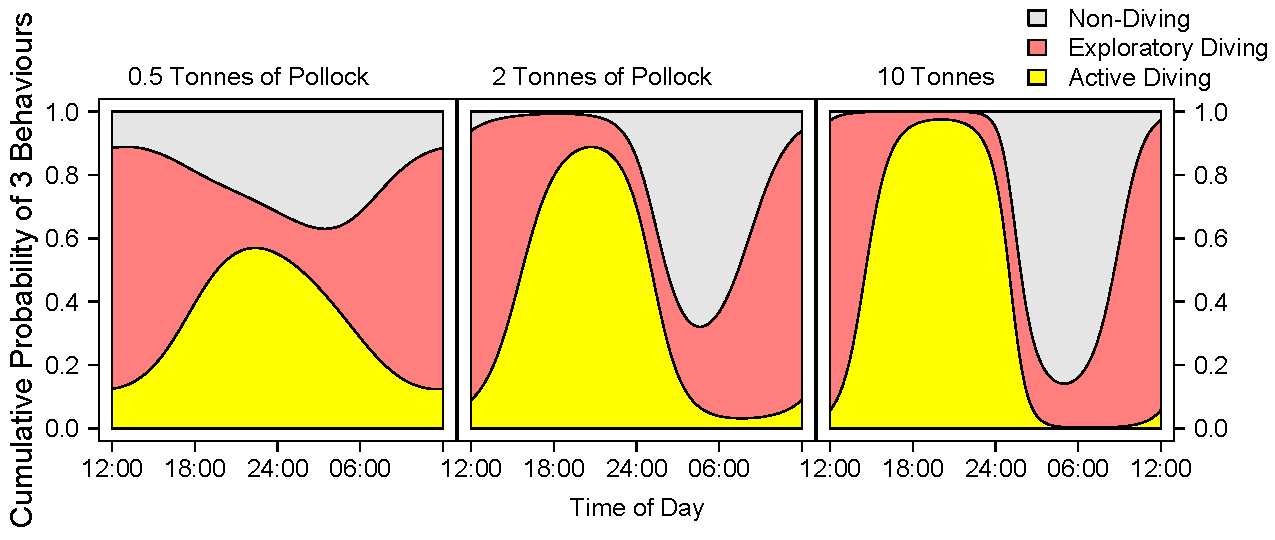
\includegraphics[width=15.3cm]{STACKED.pdf}}
\caption{Stacked probabilities of behaviour modes $Active$ $Diving$, $Exploratory$ $Diving$, and $Non$-$Diving$ in response to time of day and increasing commercial catch size of walleye pollock. The left panel of graph shows the predicted relative probabilities of behaviours in areas of small-sized walleye pollock hauls (0.5 tonnes), the middle panel shows predicted relative probabilities of behaviours in areas of medium-sized hauls (2 tonnes), and the right panel shows predicted relative probabilities of behaviour in areas of larger-sized hauls of pollock (10 tonnes). Note that the $x-$axis depicts time of day where the axis starts and finishes at noon to highlight the maximum amplitude of active foraging (in $yellow$) that happens at night. }
\label{f:STACKED}  
\end{figure} 


% Talk about the $phase$, $amplitude$ of time as a sinusoidal function. 
\subsubsection{Time $\times$ Pollock}

Figure (\ref{f:STACKED}) shows one daily cycle of behaviour in response to changes in time of day and commercial haul size of walleye pollock.   This figure highlights the increase in relative probability of engaging in active dive behaviours in response to increasing weights of pollock catch. This is accompanied by a near-zero probability of non-dive behaviours during those times of active diving in high catch areas. One caution in the  interpretation of this figure is that our model does not predict the length of time that the northern fur seals engage in particular behaviours, but rather predicts the probability of a behaviour beginning at various times of the day. 

The interpretation of the regression coefficients that correspond to time of day are from Equation (\ref{eq:CIRCLE}). This translation of time is a $1^{\rm{st}}$-order Fourier expansion, which limits the functional form to a sinusoidal curve with a period of 24 hours. Within this restriction, the model suggests the peak in the start of exploratory dive behaviours is around noon. It suggests fur seals are most likely to begin active diving behaviours at just past 8:00 in the evening, and most likely to end diving and begin non-diving behaviours around 5:00 in the morning. 
Comparing results for a haul size of 10 $t$ vs. 0.5 $t$ suggests there is a higher probability of starting active dive behaviours sooner in the evening, and hence a lower (near-zero) probability of non-dive behaviours at that time. 


\subsection{Convergence and Sensitivity}
The length of chain (1,000,000 samples) and the rate of decimation (every $50^{th}$ sample was selected to ensure full sampling of the posterior. However, for a subset of covariate models we were unable to obtain satisfactory convergence (e.g. models containing covariates the following covariates: sea surface temperature and wind; these results were omitted from Table \ref{t:TWO}). 

For the model with the best fit diagnostics (Time x Pollock), some of the fur seals did not have enough information in the covariates to identify both the latent unobserved covariate $\bm{X}_i$ and the estimate of measurement error, $\bm{\sigma}_{iU}^2$. We experimented widely with different parameter values for the prior for $\bm{\sigma}_{iU}^2$, and found that this prior not only affected convergence but also informed the location of posteriors for higher level parameters. The more restrictive the prior we put on the variance of the covariate error, the greater the coefficient effect and the poorer the model fit ($AIC$ was larger). For example, a variance of zero implies a model without measurement error in the covariates, and the effect of including the error in the covariate measure is that this pulls the magnitude of the associated parameter estimate towards zero, as well as increasing the uncertainty around that estimate. In our implementation, %we selected a diffuse prior for $\bm{\sigma}_{U}$, but put rejected posterior samples.
to allow for identification in those tracks with weakly identifiable for $\bm{\sigma}_{iU}$ and $\bm{X}_i$, we opted to reject any posterior samples of $\bm{\sigma}_{iU}$ that were greater than $5$ standard deviations from the expected value of the prior distribution. Since the selected prior distribution was diffuse, this was not a restrictive condition except for two fur seal tracks, Tracks 1 and 10.2. As the priors for each $\sigma_{iU}^2$ are independent priors, this restriction on the magnitude of the measurement error will not directly affect the measurement error estimates of the other fur seal's data. In other applications, careful examination of the prior specification may impose enough constraint to allow for identification, without restricting variance components.  

\subsection{Kullback-Leibler (KL) divergence and sample size}
Central to the Bayesian paradigm is the notion that as the data quantity and quality increase, the posterior is less sensitive to prior assumptions (Cressie et al. 2009). The results in Figure (\ref{f:KLdiv2}) summarizing the $KL$ divergence simulation described in Section (\ref{s:KL}) show there is an important gain in model performance as the number of tagged fur seals approaches 30, after which the $KL$ divergence becomes a relatively flat function. These results therefore suggest that having data collected from $\sim 30$ tagged northern fur seals would provide dependable posterior predictive inference, and that our sample size is too small for the data to assume such a dominant role in the assessment of how these spatial at-sea covariates affect northern fur seal behaviour (as one might suspect with only eleven tracks). 

\begin{figure}
\centerline{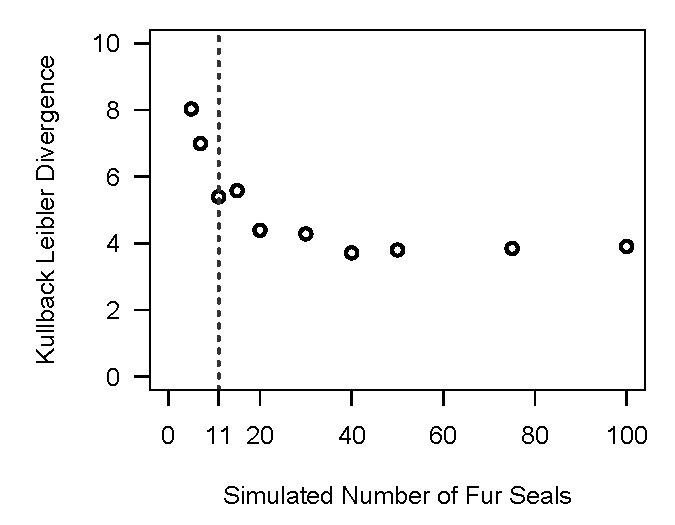
\includegraphics[width=11.3cm]{KLdiv2.pdf}}
\caption{Effect of increasing sample size on Kullback-Leibler  ($KL$) divergence for one selected population-level parameter $B_{12}$. A $KL$ divergence is 0  if and only if the posterior distribution for a simulated dataset is identical to the model from which it was generated.  The dashed vertical line at $11$  corresponds to the sample size for this study.}
\label{f:KLdiv2}  
\end{figure} 

\section{Discussion}
\label{s:DISCUSSION}

\hilight{We'll leave the discussion for now}

\hilight{ but as you go through make a running list of items and results and issues that you deem significant}. 

\hilight{check for latest and most relevant references in animal movement and Bayesian}

The hierarchical Bayesian framework used in this analysis has permitted us to significantly relate dive behaviours to the temporal and spatial fields through which lactating northern fur seals must forage in the eastern Bering Sea. We have established relationships between three distinct dive behaviours observed in lactating northern fur seals to the time of day and  measures of walleye pollock abundance around St. Paul Island, Alaska. Our analysis has shown that the interaction of time and prey abundance provides interesting insights into the organization of dive behaviours around a 24 hour, diel pattern. 

\subsubsection{Northern Fur Seals exhibit a broad foraging range} % NORDSTROM'S PAPER 
Our data were collected during the summer pupping seasons when female northern fur seals are nourishing pups and tied to a central place. This limits their effective foraging range in both time spent away, and distance traveled from the natal rookery of their dependent pup. Female northern fur seals in this study embarked on relatively long pelagic journeys averaging 279 km in linear distance from the rookery, and lasting from 5.5 to 11.2 days. This number is consistent but slightly longer than the linear distances reported in Nordstrom et al. 2013 (228 km) and Goebel et al. 1991 (200 km), and the length of time of the foraging trip is consistent with reported lengths from other studies (e.g. Gentry and Holt 1986, Nordstrom et al. 2013; from 1 to 14 days). Predictable food is thought to drive seasonal movements because pup survival depends on the amount of food available to parents for building body reserves prior to provisioning their offspring. %(Sinclair 1983). 
Therefore within a broad range of a central place, foraging habitat is selected in which they must get energy to feed themselves and their pup while still returning to the rookery in time to feed a waiting pup. 


All of the fur seals showed directional movement, but the foraging tracks of our tagged females were unconstrained and at the broadest scale did not appear collectively to prefer any one region around St. Paul Island. Individuals may, however, have such preferences. The one female for which we had two consecutive tracks went to a similarly located feeding area off-shelf in both foraging trips.  Call et al. (2008) similarly showed that 27 of 36 female fur seals with repeated recorded trips tended to travel to the same type of site following the same general direction they used in each of their previous trips. This implies that fur seals know where they are going, and suggests they may adopt a strategy of returning to the same places as used previously to forage for as long as this strategy is successful. However, none of our tracks, or those recorded by other researchers, showed consensus among the fur seals about where to feed, as none of the tracks showed fur seals traveling to a single location before swimming directly back to nurse their pups. Rather the 3-dimensional dive profiles (e.g. Figure \ref{f:D3Christina}) and horizontal behaviour maps (e.g. Figure \ref{f:MAP4}) showed consistent changes in diving behaviours throughout the at-sea foraging trips with active and exploratory dive behaviours distributed over much of the paths they swam.  In other words, there was no single grocery store or hot spot where the fur seals spent concentrated time. In other studies, northern fur seals from Reef Rookery have been found to use all hydrographic domains around St. Paul Island (eg. Robson et al. 2004), including both on-shelf and off-shelf habitats (Loughlin et al. 1987, Goebel et al. 1991, Sterling and Ream 2004, Call et al. 2008), and scat samples from the same rookery contained both on-shelf (e.g. walleye pollock, Pacific herring) and off-shelf species (e.g. myctophids; Zeppelin and Orr 2010). The lactating fur seals in this study also appear to be constantly on the move, actively feeding and exploring the ocean as they traveled through broad regions of the Bering Sea. 

\subsubsection{Persistence}
We do not know what the animals we tracked were seeking or what they caught during their foraging trips. However, juvenile walleye pollock of year-classes 0 to 5 are the most common prey in both stomach and scat diet studies (Perez and Bigg 1986, Sinclair et al. 1994, Sinclair et al. 1996, Gudmundson et al. 2006, Zeppelin and Ream 2006), and walleye pollock comprised 89.3\% of fur seal diet measured in scats collected within a month of our 2006 tagged females foraging trips from Reef Rookery (Zeppelin and Orr 2010).  We found that in at-sea locations with more abundant walleye pollock, northern fur seals were more likely to be actively diving, particularly if those locations overlapped with the nighttime.  It is unlikely that our source for the horizontal distribution and abundance of walleye pollock, which was the US Department of Commerce domestic observer data of the Alaska groundfish industry aggregated over both time and space,  %(or more generally, done at some scale in every analysis)
is directly measuring the real-time abundance of prey that the fur seals actually encountered along their foraging route at any single location. It is more likely that our measure of walleye pollock abundance represents a persistent horizontal feature that is attractive to foraging northern fur seals, but not a very accurate measure of prey availability. Likewise, Nordstrom et al. (2013) linked foraging of northern fur seals to oceanic surface fronts (eddies and filaments) and Kuhn (2011) to thermocline depth; features that may also be proxies for the horizontal and vertical distribution of prey species. 
Hence, available evidence indicates that fur seals forage more heavily in areas where either commercial catch data (this study) or oceanographic conditions (Kuhn 2011, Nordstrom et al. 2013) point to increased prey abundance. As well,  individuals tend to return to the same general area on successive foraging trips, from where they have no trouble finding the way back to the rookery. Hence, they certainly navigate successfully over hundreds of kilometres in the Bering Sea. Yet little is known to date about the extent to which they can identify potentially persistent foraging ``hot-spots'' in advance. 

\subsubsection{Competition with Fisheries}
In this study we did not include any direct measure of the bycatch of juvenile pollock in the commercial fishery, nor did we have any small scale evidence that commercial boats were fishing at the same time and location as our tagged females, thus we cannot draw conclusions about the potential for competition occurring between the commercial fishery and northern fur seals. However, we can say that being in the same area where fishing occurred would not necessarily imply competitive interactions unless it was known that the fur seals were feeding on the same fish targeted by the fishery, and whether the abundance of that target prey was limited. Evidence suggests that juvenile pollock of year-class 0 to 5 are preferred by foraging fur seals (Gudmundson et al. 2006, Zeppelin and Ream 2006), which are typically smaller than the $>40$ cm adults taken by the commercial fishery (Ianelli et al. 2007). However, inter-year variability of pollock can be as high as two orders of magnitude (1.7 t/km$^2$ in 2004, 328 t/km$^2$ in 2007 for the same region; Sigler et al. 2012). In anomalous years with poor juvenile survival combined with poor persistence of the available prey, it could be difficult for foraging females to find prey.  


\subsubsection{Dive types}
Our analysis is built upon the numerical properties of an AR-2 movement model to describe dives in terms of foraging behaviour rather than focusing on the depth at which the dives were, or the tortuosity of the at-sea path. The AR-2 process provides a mechanistic way of categorizing dive types, that is based around interpretable movement signatures, and therefore is exempt from arbitrary classification such as those distinguishing dive types based on depth (e.g. Gentry et al. 1986, Goebel 2002). Furthermore, the mechanistic approach protects us from limitations of other studies where deeper dives associated with foraging at or near the bottom were observed when fur seals were moving in straight lines and not identified as the typical tortuous paths of foraging regions (eg. Nordstrom et al. 2013, Benoit-Bird 2013a, Benoit-Bird 2013b). 
 
Each of the three behavioural modes described by dive types has an intuitive movement interpretation. Shallow, repeated dives with short surface-time intervals, as well as deeper, repeated $U$-shaped dives with comparatively longer surface recovery times are well described by the solutions of a periodic AR-2 process. $U$-shaped dives have been attributed to foraging behaviours in an array of top marine predators such as gray seals (Austin et al. 2006), southern elephant seals (Gallon et al. 2013), Australian fur seals (Arnould and Hindell 2001), harbour seals (Baechler et al. 2002), Gentoo Penguins (Wilson et al. 1996), and others. When the surface time between dives is longer but the vertical profile of the dive is more $V$-shaped, the solutions reflect a correlated random walk without a periodic component. It is less clear what the underlying motivation for intermittent $V$-shaped dives is, but others have attributed them to foraging on larger pelagic fish or squid in northern gannets (Garthe et al. 2000), or non-foraging activities, including predator avoidance, and explorations (Bengston and Stewart 1992). Non-diving and non-foraging behaviours such as resting, sleeping, grooming and surface transiting are described in the solution space as uncorrelated white noise. 

%They (Benoit-Bird13b) found deeper dives occurred at night, compared to the day, while others have found the opposite (e.g. Call et al. 2008 -- not sure if this is true). Depth-derived characteristics are not reliable indicators of foraging. 


\subsubsection{Diel pattern}

Modeling results depicted in Figure (\ref{f:STACKED}) highlight the strength of the diel pattern in foraging northern fur seals, and that the dive pattern the female engages in is that which best fits her prey environment. For example, we found that females showed strong preferences for active diving at night, while preferring non-dive behaviours such as resting or transiting in the mornings. Afternoons were typically associated with exploratory $V$-shaped dive behaviours. The model suggests that nighttime is characterized by repetitive dives of active feeding (or an AR-2 periodic solution). 
Kuhn et al. (2010) proposed that shallow foraging bouts at night may be related to juvenile walleye pollock's nighttime migrations to the surface as they follow vertically migrating zooplankton. 

It should be energetically advantageous to the northern fur seal to be able to catch prey at shallower depths, resulting in a shorter chase, and possibly also allowing the fur seal to keep physical contact with the school of prey. Northern fur seals may therefore prefer epipelagic (shallow) diving, and only transition into deeper $U$-shaped foraging dives when epipelagic resources in an area are scarce. For example, deeper foraging behaviour has been associated with fur seals targeting concentrated groups of juvenile pollock at the thermocline (Kuhn 2011, Nordstrom et al. 2013). If northern fur seals are spatially aware of broad-scale suitable feeding areas based on prior experience or some other knowledge, then it is possible they could reduce search time and energetic costs of foraging by anticipating changes in broad scale prey density and positioning themselves strategically at optimal foraging locations come nightfall. 

\subsubsection{Data requirements}
These eleven fur seal foraging trips generated some useful, basic insight into at-sea behavioural patterns across time and space. The Kullback-Leibler values of Figure (\ref{f:KLdiv2}) suggest that another 10 to 20 tracks would have generated useful further precision. We also anticipate that other oceanographic information on, for example, frontal eddies and filament locations, could provide valuable further insight into the association between fur seals and the Bering Sea environment. Within the hierarchical structure, it would be interesting to link the foraging behaviour characteristics of the maternal fur seal to her pup weight gains, as well as residency times and other life history characteristics that would contribute to our understanding of pup survival. 

\section{Conclusions}

\hilight{No need for separate conclusions. Add to Discussion}

Our analysis did not attempt to answer the question of where in the ocean did the fur seals chose to forage relative to not forage. With only 11 tracks over an area with a radius of $>200 \,\,km$ (or area $>125,000$ $km^2$), this would have been too ambitious. Instead we answer the conditional question, ``Given that the fur seal swam through this location, can we predict its most likely behaviour based on a set of local environmental variables''. Using a hierarchical Bayesian approach, we were able to link together northern fur seals that went to disparate regions of the eastern Bering Sea, with widely  variable information about their underlying environmental fields into a single model that informed us about the expected behaviour of a population of maternal, female northern fur seals at Reef Rookery on St. Paul Island. Our analysis has focussed on three typical fur seal behaviours, and how these behaviours are associated with time of day, and a set of environmental data. The approach and analysis presented here is to use hierarchical Bayesian modelling to bring together coarse estimates of the at-sea environment, and the dynamics of fur seal behaviour through identification of variable-length segments of coherent behaviours. In this, we have successfully shown that northern fur seal behaviour actively forage more at night, and in areas where their preferred prey species, juvenile walleye pollock, appears to be more abundant. 


% --------------------------------------------------------------------------------------------------------------------

\newpage
\section*{Acknowledgements}

The authors thank so and so for some helpful suggestions, for a critical reading of the original version of the
paper, and an anonymous referee for very useful comments that improved the presentation of the paper.

\begin{thebibliography}{}
\label{s:LIT3}

\bibitem[Agresti(1990)]{b1}
Agresti, A. 1990. Categorical Data Analysis. John Wiley and Sons, New York. pp 405.

\bibitem[Akaike(1973)]{b2}
Akaike, H. 1973. Information theory and an extension of the maximum likelihood principle. Second International Symposium on Information Theory, Academiai Kiado, Budapest, pp. 267-281.

\bibitem[Amante et~al.(2009)]{b3}
Amante, C., and B.W. Eakins. 2009. ETOPO1 1 Arc-Minute Global Relief Model: procedures, data sources and analysis. NOAA Technical Memorandum NESDIS NGDC-24, 19pp.


\bibitem[Antonelis et~al.(1997)]{b5}
Antonelis, G.A., E.H. Sinclair, R.R. Ream, and B.W. Robson. 1997. Inter-island variability in the diet of female northern fur seals ($Callorhinus$ $ursinus$) in the Bering Sea. Journal of Zoology, London, 242: 435-451.

\bibitem[Arnould and Hindell(2001)]{b6}
Arnould, J.P.Y. and M.A. Hindell. 2001. Dive behaviour, foraging locations, and maternal attendance patterns of Australian fur seals ($Arctocephalus$ $pusillus$ $doriferus$). Canadian Journal of Zoology, 79: 35-48.

\bibitem[Austin et~al.(2006)]{b7}
Austin, D., W.D. Bowen, J.I. McMillan, and S.J. Iverson. 2006. Linking movement, diving, and habitat to foraging success in a large marine predator. Ecology, 87: 3095-3108.

\bibitem[Baechler et~al.(2002)]{b8}
Baechler, J., C.A. Beck, and W.D. Bowen. 2002. Dive shapes reveal temporal changes in the foraging behaviour of different age and sex classes of harbour seals ($Phoca$ $vitulina$). Canadian Journal of Zoology, 80: 1569-1577.

\bibitem[Bailey et~al.(2009)]{b9}
Bailey, H., B.R. Mate, D.M. Palacios, L. Irvine, S.J. Bograd, and D.P. Costa. 2009. Behavioural estimation of blue whale movements in the Northeast Pacific from state space model analysis of satellite tracks. Endangered Species Research, 10: 93-106.

\bibitem[Banerjee et~al.(2004)]{b10}
Banerjee, S., B.P. Carlin, and A.E. Gelfand. 2004. Hierarchical Modeling and Analysis for Spatial Data. Chapman \& Hall/CRC, Boca Raton.

\bibitem[Bayarri and Berger(2000)]{b11}
Bayarri, M.J. and J.O. Berger. 2000. $P$-values for composite null models. Journal of the American Statistical Association, 95(452): 1127-1142.

\bibitem[Behrenfeld and Galkowski(1997)]{b12}
Behrenfeld, M.J. and P.G. Galkowski. 1997. Photosynthetic rates derived from satellite-based chlorophyll concentration.
Limnology  and Oceanography, 42: 1-20, \\doi:10.4319/lo.1997.42.1.0001

\bibitem[Bekker(1986)]{b13}
Bekker, P.A. 1986. Comment on identification in the linear errors in variable model. Econometrica 54 (1): 215-217.

\bibitem[Bengston et~al.(1985)]{b14}
Bengston, J.L., R.L. Merrick, and T.R. Loughlin. 1985. Radio-tracking studies, St. Paul Island, Alaska. $In$ Fur seal investigations, 1985. Edited by P. Kozloff and H. Kajimura. NOAA Tech. Memo., NMFS F/NWC-146. Pp. 104-106.

\bibitem[Benoit-Bird et~al.(2013a)]{b15}
Benoit-Bird, K.J., B.C. Battaile, C.A. Nordstrom, and A.W. Trites. 2013. Foraging behaviour of northern fur seals closely matches the hierarchical patch scales of prey. Marine Ecology Progress Series, 479: 283-302.

\bibitem[Benoit-Bird et~al.(2013b)]{b17}
Benoit-Bird, K.J., B.C. Battaile, S.A. Heppell, B. Hoover, D. Irons, N. Jones, K.J. Kuletz, C.A. Nordstrom, R.Paredes, R.M. Suryan, C.M. Waluk, and A.W. Trites, 2013. Prey Patch Patterns Predict Habitat Use by Top Marine Predators with Diverse Foraging Strategies. PloS ONE, 8(1), e53348.

\bibitem[Berkson(1950)]{b18}
Berkson, J. 1950. Are there two regressions? Journal of the American Statistical Association, Vol. 45, No. 250, pp. 164-180.

\bibitem[Berliner(1996)]{b19}
Berliner, L.M. 1996. Hierarchical Bayesian time-series models. Fundamental Theories of Physics, 79: 15-22.

\bibitem[Bestley et~al.(2013)]{b20}
Bestley, S., I.D. Jonsen, M.A. Hindell, C. Guinet, and J.-B. Charrassin. 2013. Integrative modelling of animal movement: $in$ $situ$ habitat and behavioural information for a migratory marine predator. Proceedings of the Royal Society, Series B., 280(1750):  1:19.

\bibitem[Block et~al.(2011)]{b21}
Block, B.A., I.D. Jonsen, S.J. Jorgensen, A.J. Winship, S.A. Shaffer, S.J. Bograd, E.L. Hazen, D.G. Foley, G.A. Breed, A.-L. Harrison, J.E. Ganong, A. Swithenbank, M. Castleton, H. Dewar, B.R. Mate, G.L. Shillinger, K.M. Schaefer, S.R. Benson,	 M.J. Weise, R.W. Henry and D.P. Costa. 2011. Tracking apex marine predator movements in a dynamic ocean. Nature, 475: 86-90.

\bibitem[Bowler and Benton(2005)]{b22}
Bowler, D.E. and T.G. Benton. 2005. Causes and consequences of animal dispersal strategies: relating individual behaviour to spatial dynamics Biological Reviews, 80: 205-225.


\bibitem[Breed et~al.(2009)]{b23}
Breed, G.A., I.D. Jonsen, R.A. Myers, W.D. Bowen, and M.L. Leonard. 2009. Sex-specific, seasonal foraging tactics of adult grey seals (Halichorerus grypus) revealed by state space analysis. Ecology. 90: 3209-3221.

\bibitem[Breed et~al.(2012)]{b24}
Breed, G.A. D.P. Costa, I.D. Jonsen, P.W. Robinson, and J. Mills-Flemming. 2012. State-space methods for more completely capturing behavioral dynamics from animal tracks. Ecological Modelling, 235-236: 49-58. 

\bibitem[Brooks and Gelman(1998)]{b25}
Brooks, S.P. and Gelman, A. 1998. General methods for monitoring convergence of iterative simulations. Journal of Computational and Graphical Statistics, 7: 434-455.

\bibitem[Burnham and Anderson(2001)]{b26}
Burnham, K.P., and D.R. Anderson. 2001. Kullback-Leibler information as a basis for strong inference in ecological studies. Wildlife Research. 28: 111-119.

\bibitem[Calder et~al.]{b27}
Calder, C.A., M. Lavine, P. Mueller, and J.S. Clark. 2003. Incorporating multiple sources of stochasticity in populations dynamic models. Ecology, 84: 1395-1402. 


\bibitem[Call et~al.]{b28}
Call, K.A., R.R. Ream, D. Johnson, J.T. Sterling, and R.G. Towell. 2008. Foraging route tactics and site fidelity of adult female northern fur seal ($Callorhinus$ $ursinus$) around the Pribilof Islands. Deep-Sea Research Part II. 55(16): 1883-1896.

\bibitem[Carlin and Louis(2000)]{b29}
Carlin, B., and T.A. Louis. 2000. Bayes and empirical Bayes methods for data analysis (2$^\textrm{nd}$ ed.). 418 pp.

\bibitem[Carroll et~al.]{b30}
Carroll, R.J., D. Rupert,  L.A. Stefanski, and C.M. Crainiceanu. 2006. Measurement Error in Nonlinear Models A Modern Perspective. ($2^{nd}$ ed.) Boca Raton, FL: Chapman \& Hall/CRC. 455 pp. %(ISBN 1-58488-633-1. xxviii + 455 pp.)

\bibitem[Clyde(2000)]{b31}
Clyde, M.A. 2000. Model uncertainty and health effect studies for particulate matter. Environmetrics, 11:745:763. 


\bibitem[Cressie et~al.]{b32}
Cressie, N., C.A. Calder, J.S. Clark, J.M. Ver Hoef, and C.K. Wikle. 2009. Accounting for uncertainty in ecological analysis: the strengths and limitations of hierarchical statistical modelling. Ecological Applications, 19(3): 553-570.

\bibitem[Dempster(1974)]{b33}
Dempster, A.P. 1974. The direct use of likelihood for significance testing. $In$ Proceedings of Conference on Foundational questions in statistical inferences, ($ed.$ O. Barndorff-Nielsen, P. Blaesild, and G. Schou), pp.335-352. Department of Theoretical Statistics: University of Aarhus. 

\bibitem[Dey et~al.]{b34}
Dey, D.K., A.E. Gelfand, T.B. Swartz, and P.K. Vlachos. 1998. A simulation-intensive approach for checking hierarchical models. Test, 7(2): 325-346.

\bibitem[Fauchald(2003)]{b35}
Fauchald, P., and T. Tveraa. 2003. Using first passage time in the analysis of area-restricted search and habitat selection. Ecology. 84: 282-288.

\bibitem[Fauchald]{b36}
Fauchald, P., and T. Tveraa. 2006. Hierarchical patch dynamics and annual movement pattern. Oecologia. 149: 383-395.

\bibitem[Fidell]{b37}
Fidell, B.G., and L.S. Tabachnick. 2006. Using multivariate statistics (5th ed.). Boston: Allyn \& Bacon. 1008 pp.

\bibitem[Gallon et~al.]{b38}
Gallon, S., F. Bailleul, J.-B. Charrassin, C. Guinet, C.-A. Bost, Y. Handrich and M. Hindell. 2013. Identifying foraging events in deep diving southern elephant seals, $Mirounga$ $leonina$, using acceleration data loggers. Deep-Sea Research II, 88-89: 14-22.

\bibitem[Garthe et~al.]{b39}
Garthe, S., S. Benvenuti and W.A. Montevecchi. 2000. Pursuit plunging by northern gannets ($Sula$ $bassana$) ``feeding on capelin ($Mallotus$ $villosus$)''. Proceedings of the Royal Society B,  267(1454): 1717-1722.

\bibitem[Gelfand]{b40}
Gelfand, A.E., and A.F.M. Smith. 1990. Sampling based approaches to calculating marginal densities. Journal of the American Statistical Association 85: 398-409.

\bibitem[Gelfand]{b41}
Gelfand, A.E. 2012. Hierarchical modelling for spatial data problems. Spatial Statistics, 1: 30-39.


\bibitem[Gelman]{b42}
Gelman, A., J.B. Carlin, H.S. Stern, and D.B. Rubin. 2004. Bayesian data analysis ($2^{\textrm{nd}}$ ed.). Boca Raton, FL: CRC Press. 668 pp.

%\item[]
%Gelman, A., X.-L. Meng, H. Stern. 1996. Posterior predictive assessment of model fitness via realized discrepancies (with discussion). Statistica Sinica, 6: 733-807.


\bibitem[Gelman et~al.]{b43}
Gelman, A., J.B. Carlin, H.S. Stern, and D.B. Rubin. 2004. Bayesian data analysis ($2^{nd}$ ed.). Boca Raton, FL: CRC Press. 668 pp.

\bibitem[Gelman and Rubin(1992)]{b44}
Gelman, A., and D.B. Rubin. 1992. Inference from iterative simulation using multiple sequences (with discussion). Statistical Science, Vol 7, 457-511. 

\bibitem[Geman]{b45}
Geman, S., and D. Geman. 1984. Stochastic relaxation, Gibbs distributions, and the Bayesian restoration of images. IEEE Transactions on Pattern Analysis and Machine Intelligence, 6: 721-741.


\bibitem[Gentry]{b46}
Gentry, R.L., and J.R. Holt. 1986. Attendance behavior of northern fur seals. $In$ Fur seals, maternal strategies on land and at sea. Edited by R. L. Gentry and G. L. Kooyman. Princeton University Press, Princeton, NJ, pp. 41-60.


\bibitem[Gentry et~al.]{b47}
Gentry, R.L., G.L. Kooyman, and M.E. Goebel. 1986. Feeding and diving behavior of northern fur seals. Pp. 61-78. $In$ R. L. Gentry and G. L. Kooyman ($eds.$). Fur seals: maternal strategies on land and at sea, Princeton University Press, Princeton.

\bibitem[Gilks et~al.]{b48}
Gilks, W.R., S. Richardson, and D.J. Spiegelhalter. 1995. Markov Chain Monte Carlo in Practice. Chapman \& Hall/CRC Interdisciplinary Statistics, 497pp.

\bibitem[Gimenez et~al.]{b49}
Gimenez, O., S.J. Bonner, R. King, R.A. Parker, S.P. Brooks, L.E. Jamieson, V. Grosbois, B.J.T. Morgan and L. Thomas. 2009. WinBUGS for Population Ecologists: Bayesian Modeling Using Markov Chain Monte Carlo Methods. \textit{In} D.L. Thomson, E.G. Cooch, and M.J. Conroy. (\textit{Eds.}), Modeling Demographic Processes in Marked Populations. \textit{In Series} Environmental and Ecological Statistics. Springer US, 883-915pp. 


\bibitem[Goebel et~al.]{b50}
Goebel, M., J. Bengtson, R. DeLong, R. Gentry, and T.R. Loughlin. 1991. Diving patterns and foraging locations of female northern fur seals. Fishery Bulletin, 89: 171-179.

\bibitem[Goebel]{b51}
Goebel, M.E. 2002. Northern fur seal lactation, attendance and reproductive success in two years of contrasting oceanography. PhD thesis, University of California, Santa Cruz. 227 pp.


\bibitem[Gudmundson et~al.]{b52}
Gudmundson, C.J., T.K. Zeppelin, and R.R. Ream. 2006. Application of two methods for determining diet of northern fur seals (Callorhinus ursinus). Fishery Bulletin, 104: 445-455.

\bibitem[Gustafson]{b53}
Gustafson, P. 2004. Measurement error and misclassification in Statistics and Epidemiology: Impacts and Bayesian adjustments Chapman \& Hall/CRC.

\bibitem[Harcourt]{b54}
Harcourt, R., and L. Davis. 1997. The use of satellite telemetry to determine fur seal foraging areas. Pp. 137-142. $In$ M. Hindell and C. Kemper (eds.). Marine Mammal Research in the Southern Hemisphere Volume 1: Status, Ecology, and Medicine, Surrey Beatty \& Sons.

\bibitem[Harris]{b55}
Harris, K.J., and P.G. Blackwell. 2013. Flexible continuous-time modelling for heterogeneous animal movement. Ecological Modelling, 255: 229-237.

\bibitem[Hastings(1970)]{b56}
Hastings, W. 1970. Monte Carlo sampling methods using markov chains and their applications. Biometrika, 57(1):97-109.



\bibitem[Herrmann]{b56}
Herrmann, E. 2003. Lokern: An R package for kernel smoothing.  

%\item[]
%Johnson, J.B. and K.S. Omland. 2004. Model selection in ecology and evolution. Trends in Ecology and Evolution, 19(2): 101-108.

\bibitem[Johnson]{b57}
Johnson, V. 2004. A Bayesian $\chi^2$-test for goodness of �t. Annals of Statistics, 32(6): 2361-2384.

\bibitem[Johnson]{b58}
Johnson, J.B. and K.S. Omland. 2004. Model selection in ecology and evolution. Trends in ecology \& evolution, 19(2):  101-108. 

\bibitem[Johnson et~al.]{b59}
Johnson, D.S., J.M. London, M.-A. Lea, and J.W. Durban. 2008. Continuous-time correlated random walk model for animal telemetry data. Ecology, 89(5): 1208-1215.

\bibitem[Jonsen et~al.]{b60}
Jonsen, I.D., R.A. Myers, and J.M. Flemming. 2005. Robust state space modeling of animal movement data. Ecology, 86: 2874-2880.

\bibitem[Jonsen et~al.]{b61}
Jonsen ID, R.A. Myers, and M.C. James. 2007. Identifying leatherback turtle foraging behaviour from satellite-telemetry using a switching state space model. Marine Ecology Progress Series, 337: 255-264.

\bibitem[Jonsen et~al.]{b62}
Jonsen, I.D., M. Basson, S. Bestley, M.V. Bravington, T.A. Patterson, M.W. Pedersen, R.Thomson, U.H. Thygesen, and S.J. Wotherspoon. 2012. State-space models for bio-loggers: A methodological road map. Deep Sea Research II \\(http://dx.doi.org./10.1016/j.dsr2.2012.07.008): 1-13.

\bibitem[Kass et~al.]{b63}
Kass, R.E.,  B.P. Carlin, A. Gelman, and R.M. Neal. 1998. Markov Chain Monte Carlo in Practice: A Roundtable Discussion. American Statistician, 52: 93-100.

\bibitem[Kareiva]{b64}
Kareiva, P., and G. Odell. 1987. Swarms of predators exhibit "preytaxis" if individual predators use area-restricted search. American Naturalist, 130: 233-270.

\bibitem[Kim]{b65}
Kim, C., and C. Nelson. 1999. State-space models with regime switching: classical and Gibbs sampling approaches with applications. MIT Press Books. 

\bibitem[Kuhn et~al.]{b66}
Kuhn, C.E., Y. Tremblay, R.R. Ream, and T.S. Gelatt. 2010. Coupling GPS tracking with dive behavior to examine the relationship between foraging strategy and �ne-scale movements in northern fur seals ($Callorhinus$ $ursinus$). Endangered Species Research, 12:125-139.

\bibitem[Kuhn]{b67}
Kuhn, C.E. 2011. The in�uence of subsurface thermal structure on the diving behavior of northern fur seals ($Callorhinus$ $ursinus$) during the breeding season. Marine Biology, 158: 649-663.


\bibitem[Kullback]{b68}
Kullback, S., and R.A. Leibler. 1951. On information and sufficiency. The Annals of the Institute of Statistical Mathematics, 22: 79-86.

\bibitem[Lambert et~al.]{b37}{b69}
Lambert, P.C., A.J. Sutton, P.R. Burton, K.R. Abrams, and D.R. Jones. 2005. How vague is vague? A simulation study of the impact of the use of vague prior distributions in MCMC using WinBUGS. Statistics in Medicine, 24: 2401�2428.


\bibitem[Lee]{b70}
Lee., Y.K., and B.U. Park. 2006. Estimation of Kullback-Leibler divergence by local likelihood. The Annals of the Institute of Statistical Mathematics, 58(2): 326-340.


\bibitem[Leisch]{b78}
Leisch, F. 2004. FlexMix: A General Framework for Finite Mixture Models and Latent Class Regression in {R}. Journal of Statistical Software, 11(8): 1-18.


\bibitem[Loughlin et~al.]{b79}
Loughlin, T.R., J.L. Bengtson, and R.L. Merrick. 1987. Characteristics of feeding trips of female northern fur seals. Canadian Journal of Zoology, 65: 2079-2084.
 
 
\bibitem[Loughlin et~al.]{b80}
Loughlin, T.R., I.N. Sukhanova, E.H. Sinclair, and R.C. Ferrero. 1999. Summary of biology and ecosystem dynamics in the Bering Sea. Dynamics of the Bering Sea, 99(1999): 387�407.


\bibitem[McClintock et~al.]{b81}
McClintock, B.T., D.J.F. Russell, J. Matthiopoulos, and R. King. 2013. Combining individual animal movement and ancillary biotelemetry data to investigate population-level activity budgets. Ecology, 94(4): 838-849.

\bibitem[McCullagh]{b82}
McCullagh, P. and J.A. Nelder. 1989. Generalized Linear Models, Second Edition. Chapman \& Hall/CRC Monographs on Statistics and Applied Probability.

\bibitem[Meng]{b83}
Meng, X.L. 1994. Posterior predictive $p$-values. The Annals of Statistics, 22(3): 1142-1160.

\bibitem[Metropolis et~al.]{b84}
Metropolis, N., A.W. Rosenbluth, M.N. Rosenbluth, A.H. Teller, and E. Teller. 1953. Equation of state calculations by fast computing machines. The Journal of Chemical Physics, 21(6): 1087�1093.

\bibitem[Mitani et~al.]{b85}
Mitani, Y., K. Sato, I. Shinichiro, M.F. Cameron, D.B. Siniff, and Y. Naito. 2003. A method for reconstructing three-dimensional dive profiles of marine animals using geomagnetic intensity data: results from two lactating Weddell seals. Polar Biology, 26: 311-317.
%\item[]
%Morales, J.M., D.T. Haydon, J. Friar, K.E. Hosinger, J.M. Fryxell. 2004. Extracting more from relocation data: building movement modles as mixtures of random walks. Ecology, 85(9): 2436-2445. % NOTE THIS IS A HBM APPROACH!

\bibitem[NMFS]{b86}
NMFS. 2007. Conservation plan for the Eastern Pacific stock of northern fur seal ($Callorhinus$ $ursinus$). National Marine Fisheries Service, Juneau, Alaska. 

\bibitem[NMFS]{b87}
NMFS. 2012. National Observer Program Annual Report � FY 2011, NOAA Tech. Memo. NMFS F/SPO-123, 36 pp. 


\bibitem[Nordstrom et~al.]{b88}
Nordstrom, C.A., B.C. Battaile, C. Cott\'{e}, and A.W. Trites. 2013. Foraging habitats of lactating northern fur seals are structured by thermocline depths and submesoscale fronts in the eastern Bering Sea. Deep-Sea Research II, \\http://dx.doi.org/10.1016/j.dsr2.2012.07.010

\bibitem[Ntzoufras]{b89}
Ntzoufras, I. 2009. Bayesian modeling using WinBUGS. Hoboken, NJ: Wiley, 492pp.


\bibitem[Patterson et~al.]{b90}
Patterson, T.A.,  M. Basson, M.V. Bravington, and J.S. Gunn. 2009. Classifying movement behaviour in relation to environmental conditions using hidden Markov models. Journal of Animal Ecology. 78: 1113-1123.

\bibitem[Perez]{b91}
Perez, M.A., and M.A. Bigg. 1986. Diet of northern fur seals, $Callorhinus$ $ursinus$, off western North America. Fishery Bulletin, 84: 957-971.

\bibitem[Pitt]{b92}
Pitt, M.A., and I.J. Myung. 2002. When a good fit can be bad. Trends in Cognitive Science, 6: 421-425.

\bibitem[Priestley]{b93}
Priestley, M.B. 2004. Spectral Analysis and Time Series. Academic Press. London. 890pp.

\bibitem[Ream et~al.]{b94}
Ream, R.R., J.T. Sterling, and T.R. Loughlin. 2005. Oceanographic features related to northern fur seal migratory movements. Deep Sea Research Part II: Topical Studies in Oceanography, 52(5), 823-843.

\bibitem[Richardson]{b95}
Richardson, S., and W.R. Gilks. 1993. A Bayesian approach to measurement error problems in epidemiology using conditional independence models. American Journal of Epidemiology, 138: 430-442.


\bibitem[Roberts]{b96}
Roberts, C.P., and G. Casella. 2005. Monte Carlo statistical methods. Second edition. Springer, New York, New York, USA.

\bibitem[Roberts]{b97}
Roberts, G.O. and J.S. Rosenthal. 2009. Examples of Adaptive MCMC. Journal of Computational and Graphical Statistics, 18(2): 349-367.


\bibitem[Robson et~al.]{b98}
Robson, B. W., M. E. Goebel, J. D. Baker, R.R. Ream, T.R. Loughlin, R.C. Francis, G.A. Antonelis, and D.P.Costa. 2004. Separation of foraging habitat among breeding sites of a colonial marine predation, the northern fur seal ($Callorhinus$ $ursinus$). Canadian Journal of Zoology, 82: 20�29.

\bibitem[Royer et~al.]{b99}
Royer, F., J.M. Fromentin and P. Gaspar. 2005. A state space model to derive bluefin tuna movement and habitat from archival tags. Oikos, 109(3): 473-484.

\bibitem[Royle]{b100}
Royle, J. A., and R.M. Dorazio. 2008. Hierarchical modeling and inference in ecology: the analysis of data from populations, metapopulations and communities. Academic Press. 444pp.



\bibitem[Rubin]{b101}
Rubin, D.B. 1984. Bayesian justifiable and relevant frequency calculations for the applied statistician. The Annals of Statistics, 12: 1152-1172.

\bibitem[Rahul(1981)]{b102}
Schennach, S.M. 2004, Estimation of nonlinear models with measurement error. Econometrica, 72 (1): 33-75.

\bibitem[Shumway]{b103}
Shumway, R.H., and D.S. Stoffer. 2006. Time Series Analysis and Its Applications: With R Examples. Third Edition. Springer Texts in Statistics, New York. 575pp.


\bibitem[Sigler et~al.]{b104}
Sigler, M.F., K.J. Kuletz, P.H. Ressler, N.A. Friday, C.D. Wilson, and A.N. Zerbini. 2012. Marine predators and persistent prey in the southeast Bering Sea. Deep-Sea Research II, 65-70: 292-303.




\bibitem[Sinclair et~al.]{b105}
Sinclair, E.H., T.R. Loughlin, and W. Pearcy. 1994. Prey selection by northern fur seals ($Callorhinus$ $ursinus$) in the eastern Bering Sea. Fishery Bulletin, 92: 132-156.

\bibitem[Sinclair et~al.]{b106}
Sinclair, E.H., G.A. Antonelis, B.W. Robson, R. Ream, and T.R. Loughlin. 1996. Northern fur seal, $Callorhinus$ $ursinus$, predation on juvenile pollock, $Theragra$ $chalcogramma$. Pp. 167-178. $In$ R. D. Brodeur, P. A. Livingston, T. R. Loughlin, and A. B. Hollowed, ($eds.$). Ecology of juvenile walleye pollock, $Theragra$ $chalcogramma$: papers from the workshop "The importance of pre-recruit walleye pollock to the Bering Sea and North Pacific ecosystems" Seattle, Washington, 28-30 October 1993. U.S. Department of Commerce, NOAA Technical. Report. NMFS-126. 227 pp.


\bibitem[Spiegelhalter et~al.]{b107}
Spiegelhalter, D., A. Thomas, N. Best, and D. Lunn. 2002. WinBUGS User Manual Version 1.4. Medical Research Council Biostatistics Unit: Cambridge, UK.

\bibitem[Stephens]{b108}
Stephens, D.A., and P. Dellaportas. 1992. Bayesian analysis of generalized linear models with covariate measurement error. \textit{In} J. M. Bernardo, J. O. Berger, A. P. Dawid, and A. F. M. Smith (\textit{Eds.}), Bayesian Statistics 4 (pp. 813-820), Oxford: Oxford University Press.

\bibitem[Sterling]{b109}
Sterling, J.T., and R.R. Ream. 2004. At-sea behavior of juvenile male northern fur seals ($Callorhinus$ $ursinus$). Canadian Journal of Zoology, 82: 1621-1637.

\bibitem[Thums et~al.]{b110}
Thums, M., C.J.A. Bradshaw, and M.A. Hindell. 2011. In situ measures of foraging success and prey encounter reveal marine habitat-dependent search strategies. Ecology, 92(6): 1258-1270. 

\bibitem[Towell et~al.]{b111}
Towell, R.G., R.R. Ream, and A.E. York. 2006. Decline in northern fur seal ($Callorhinus$ $ursinus$) pup production on the Pribilof Islands. Marine Mammal Science, 22(2): 486-491.

\bibitem[Wasserman]{b112}
Wasserman, L. 2004. All of Statistics: A Concise Course in Statistical Inference. Springer, New York, 445pp.

\bibitem[Weimerskirch et~al.]{b113}
Weimerskirch, H., D. Pinaud, F. Pawlowski, and C.-A. Bost. 2007. Does prey capture induce area-restricted search. A fine-scale study using GPS in a marine predator, the wandering albatross. American Naturalist, 170: 734-743.

\bibitem[Wikle]{b114}
Wikle, C.K. 2003. Hierarchical models in environmental science. International Statistical Review, 71: 181-199.

\bibitem[Wilson et~al.]{b115}
Wilson, R.P., B.M. Culik, G. Peters, R. Bannasch. 1996. Diving behaviour of Gentoo penguins, $Pygoscelis$ $papua$; factors keeping dive profiles in shape. Marine Biology, 126: 153-162. 

\bibitem[Zeppelin]{b116}
Zeppelin, T.K., and R.R. Ream. 2006. Foraging habitats based on the diet of female northern fur seals ($Callorhinus$ $ursinus$) on the Pribilof Islands, Alaska. Journal of Zoology, 270: 565-576.

\bibitem[Zeppelin]{b117}
Zeppelin, T.K., and A.J. Orr. 2010. Stable isotope and scat analyses indicate diet and habitat partitioning in northern fur seals $Callorhinus$ $ursinus$ across the eastern Pacific. Marine Ecology Progress Series, 409: 241-253.

\bibitem[Zhang]{b118}
Zhang, H.M., J.J. Bates, and R.W. Reynolds. 2006. Assessment of composite global sampling: Sea surface wind speed. Geophysical Research Letters, 33(17).

\end{thebibliography}


% --------------------------------------------------------------------------------------------------------------------
\end{document}
% --------------------------------------------------------------------------------------------------------------------
  
  
  
\section[]{Material Description of the Envelope Predominantly Model}

If we assume that the dust grains in the envelope are predominantly of
the same kind and are in thermal equilibrium, the luminosity at
frequency $\nu$ in the infrared is given by
\begin{equation}
 L(\nu)=\mskip-12mu\int\limits_{\text{envelope}}\mskip-12mu
 \rho(r)Q_{\text{abs}}(\nu)B[\nu,T_{\text{g}}(r)]\exp [-\tau(\nu,r)]\>
 \text{d}V,
\label{eq:luminosity}
\end{equation}
 where
 $Q_{\text{abs}}(\nu)$ is the absorption efficiency at frequency $\nu$,
 $\rho(r)$ is the dust grain density,
 $T_{\text{g}}(\nu)$ is the grain temperature,
 $B[\nu,T_{\text{g}}(r)]$ is the Planck function, and
 $\tau(\nu,r)$ is the optical depth at distance {\it r\/} from the
 center of the star.
The temperature $T_{\text{g}}(r)$ is determined by the condition of energy
balance: amount of energy radiated = amount of energy absorbed. The
amount of energy absorbed at any point is proportional to the total
available energy at that point, which consists of:\pagebreak
\begin{enumerate}
 \item The attenuated and diluted stellar radiation. The attenuated and diluted stellar radiation;
 \item Scattered radiation, and
 \item Reradiation from other grains.
\end{enumerate}

The amount of energy absorbed at any point is proportional to the total
available energy at that point
\begin{itemize}
 \item The attenuated and diluted stellar radiation. The attenuated and diluted stellar radiation;
 \item Scattered radiation, and
 \item Reradiation from other grains. Reradiation from other grains.
\end{itemize}

Detailed solutions of radiative transfer in circumstellar dust
shells by \citet{b21} indicate that the effect of heating by
other grains becomes significant only at large optical depths at
the absorbing frequencies $[\tau(\text{UV})\gg 10]$, and at optical
depths $\tau(\text{UV})<1$ the grains have approximately the same
temperature that they would have if they were seeing the starlight
unattenuated and no other radiation.
\begin{description}
\item The Planck mean optical depths of circumstellar envelopes around
several RV Tauri stars.
\item The Planck mean optical depths of circumstellar envelopes around
several RV Tauri stars.
\item The Planck mean optical depths of circumstellar envelopes around
several RV Tauri stars.
\end{description}
The pure terrestrial silicates
or lunar silicates are found to be completely unsuitable to
account for the infrared emission from circumstellar dust shells
around M-type stars \citep{b21}. We assume that the absorption
efficiency $Q_{\text{abs}} (\nu)$ in the infrared varies as
$\nu^{\gamma}$. ${\gamma}=1$ appears to provide a reasonable fit
in a variety of sources \citep*{b11,b12}. Under these
circumstances the condition of energy balance implies that the
dust temperature $T_{\text{g}}$ will vary as $r^{\beta}$.

In view of the low value of the observed Planck mean optical depth for
the stellar radiation and the nature of the assumed frequency
dependence of the absorption efficiency, the extinction of the infrared
radiation by the dust envelope can be neglected. If we consider the
envelope to be spherically symmetric, (\ref{eq:luminosity}) reduces to
\begin{equation}
 L(\nu)=\!\!\int_{r_{1}}^{r_{2}}\!\!4\uppi r^2\rho(r)\> Q_{\text{abs}}(\nu)B[\nu,T_{\text{g}}(r)]\> {\text{d}}r,
\label{eq:reducelum}
\end{equation}
where $r_1$ and $r_2$ are the inner and
outer radii of the shell. For a dusty density distribution
$\rho(r)\propto r^{\alpha}$ and $r_2\gg r_1$, (\ref{eq:reducelum}) reduces to
\begin{equation}
 L(\nu)\propto \nu^{2+\gamma-Q}\int_{X_0}^{\infty}{{x^Q}\over
 {\text{e}^x-1}}\text{d}x ,
\label{eq:dusty}
\end{equation}
where, in (\ref{eq:dusty}), $Q=-(\alpha+\beta+3)/\beta$ and $X_0=(h\nu
/kT_0)$. $T_0$ represents the temperature at the inner boundary of the
dust shell where grains start condensing. In a steady radiation
pressure driven mass outflow in the optically thin case, values of
$\alpha$ lie near $-2$ \citep{b8}. $\gamma$ and $\beta$ are related by
$\beta=-2/(\gamma+4)$.

In the {\it NIFT\/} Point Source Catalog \citep[PSC;][]{b2}, the flux
densities have been quoted at the effective wavelengths 12, 25, 60 and
\hbox{100\,$\upmu$m}, assuming a flat energy spectrum $[\nu F(\nu)=1]$
for the observed sources. See Table~\ref{t:tablethree} for more
details. For each model given by equation~\ref{eq:dusty}, using the relative
system response, the color-correction factors in each of the {\it
NIFT\/} passbands were calculated and the fluxes were converted into
flux densities expected for a flat energy distribution, as assumed in
the {\it NIFT\/} PSC, so that the computed colors can be directly
compared with the colors determined from the catalog
quantities. Such a procedure is more appropriate than correcting the
{\it NIFT\/} colors for the energy distribution given by a particular
model and then comparing them with those computed by the model.

\section{An Example of Head One Color-Color Diagram An Example of Head One Color-Color Diagram}

\subsection{An Example of Head Two: Color-Color Diagram An Example of Head Two: Color-Color Diagram}
\label{ss:example}

The IR color is defined as
%\[
\begin{eqnarray*}
 [\nu_1]-[\nu_2]=-2.5\log [f(\nu_1)/f(\nu_2)],
\end{eqnarray*}
%\]
 where $\nu_1$ and $\nu_2$ are any two wavebands and $f(\nu_1)$ and
$f(\nu_2)$ are the corresponding flux densities assuming a flat energy
spectrum for the source. In Figure~\ref{f:mouse1column}, we have
plotted the [25]--[60] colors of RV Tauri stars against their
corresponding [12]--[25] colors derived from the {\it NIFT\/}
data. Filled circles represent stars of group A and open circles stars
of group B. The two sets of
near-parallel lines represent the loci of constant inner shell
temperature $T_0$ and the quantity $Q$ defined above. The models
correspond to the case of absorption efficiency $Q_{\text{abs}}(\nu)$
varying as $\nu$ (with $\gamma=1$ and hence $\beta=-0.4$). We have
omitted R Sct in Figure~\ref{f:mouse1column} because it shows a large
deviation from the average relation shown by all the other objects. R
Sct has a comparatively large excess at 60$\,\upmu$m, but the extent of
a possible contamination by the infrared cirrus \citep{b16} is
unknown. \citet{b9} found no evidence of the presence of a dust
envelope at near-IR wavelengths and the spectrum was consistent with a
stellar continuum. This explains why R Sct lies well below the mean
relation shown by stars of groups A and C between the [3.6]--[11.3]
color excess and the photometrically determined (Fe/H) \citep{b4}. R
Sct has the longest period of 140$\,$d among the RV Tauri stars
detected at far-infrared wavelengths and does the RV Tauri stars
detected at far-infrared wavelengths and does the RV Tauri stars
detected at far-infrared wavelengths and does not have the 10-$\upmu$m
emission feature seen in other objects \citep{b5,b19}. R Sct is
probably the most irregular RV Tauri star known \citep{b17}. In Web
Appendix 1, we give a derivation that shows that this is to be
expected.

The inner shell temperatures $(T_0)$ derived for the various objects
are also given in Table~\ref{t:tableone} and we find the majority
of them to have temperatures in the narrow range
400--600$\,$K. If the dependences of $Q_{\text{abs}}(\nu)$ on $\nu$ and
$\rho(r)$ on $r$ are similar in all the objects considered, then in
the color--color diagram they all should lie along a line
corresponding to different values of $T_0$ and in
Figure~\ref{f:bigmouse} we find that this is ebiomntially the case. In
view of the quoted uncertainties in the flux measurements, we cannot
attach much significance to the scatter in Figure~\ref{f:bigmouse}.

\begin{figure}
 \centerline{\includegraphics[width=2.25in]{mouse.eps}}
\caption{An example of figure caption. An example of figure
caption. An example of figure caption. An example of figure
caption.}
\label{f:mouse1column}
\end{figure}


At \hbox{100\,$\upmu$m} the infrared sky is characterized by emission,
called infrared cirrus, from interstellar dust on all spatial scales
\citep{b16}, thereby impairing the measurements at far-infrared
wavelengths. In Figure~\ref{f:shortmouse}, we have plotted the
[60]--[100] colors of the six RV Tauri stars detected at
\hbox{100\,$\upmu$m} against their [25]--[60] colors, along with the
grid showing the regions of different values for inner shell
temperature $T_0$ and the quantity $Q$, as in Figure~\ref{f:bigmouse}.
The results indicated by Figure~\ref{f:shortmouse} are consistent with
those derived from Figure~\ref{f:mouse1column}. AR Pup shows a large
excess at \hbox{100\,$\upmu$m} but, in view of the large values for the
cirrus flags given in the catalog, the intrinsic flux at
\hbox{100\,$\upmu$m} is uncertain.


\subsection{Radial Distribution of Dust}

From Figure~\ref{f:shortmouse}, it is evident that all RV Tauri stars
lie between the lines corresponding to $Q=1.5$ and 0.5. With
 \[
 \alpha=-(1+Q)\beta-3,
 \]
 these values suggest limits of $r^{-2.0}$ and $r^{-2.4}$ for the dust
density variation, indicating a near-constant mass-loss rate.
\citet{b12} has suggested that the density in the circumstellar
envelope around RV Tauri stars varies as $r^{-1}$, implying a
mass-loss rate that was greater in the past than it is currently. By
fitting a power law to the observed fluxes, such that $f(\nu)$ varies
as $\nu^q$, values of $q$ determined by him for the various objects
given in Table~\ref{t:tableone} lie in the range 0.6--1.2, with a mean
$\skew5\bar q=0.98$. The assumption of a power law corresponds to the
case of $X_0=0$ in equation (3) and hence we get
 \[
 q=2+\gamma -Q.
 \]
Since we assume that $Q_{\text{abs}}(\nu)$ varies as $\nu$, the
resulting value for $Q$=2.0. None of the objects is found to lie in the
corresponding region in the color--color diagram. Even this extreme
value for $Q$ implies a density which varies as $r^{-1.8}$.

\citet{b9} have reported that the simultaneous optical and near-IR
data of AC Her can be fitted by a combination of two blackbodies
at 5680 and 1800\,K, representing, respectively, the stellar and
dust shell temperatures, and suggested that in RV Tauri stars the
grain formation is a sporadic phenomenon and not a continuous
process. Apparently, they have been influenced by the remark by
\citet{b7} that their data in the 3.5--11$\,\upmu$m region of AC
Her indicated a dust temperature of $\sim$300\,K. We find that the
{\it K--L\/} colors given by \citet{b5} and
\citet{b9} are all consistent with each other. Surely, hot dust
($\sim$1800\,K), if present at the time of observations by
\citet{b9}, would have affected the {\it K--L\/} color
significantly. AC Her, like other members of its class, is found
to execute elongated loops in the ({\it U--B\/}), ({\it B--V\/})
plane \citep{b20}, indicating that significant departure of the
stellar continuum from the blackbody is to be expected. Further,
their data show only a marginal excess at the near-IR wavelengths.


\subsection{An Example of Head two}

\subsubsection{An example of head three comparison with oxygen and~carbon~Miras}

In Figure~\ref{f:shortmouse} we have also shown the positions of a
sample of oxygen-rich and carbon-rich Miras. We feel that the case
for the existence of hot dust around AC Her and hence for the sporadic
grain formation around RV Tauri stars is not strong. In
Figure~\ref{f:bigmouse}, we find that AC Her and RU Cen lie very close
to R Sct which, according to \citet{b9}, shows no evidence for the
presence of a hot dust envelope. At the low temperatures
characteristic of the Miras, a part of the emission at 12$\,\upmu$m
comes from the photosphere. For a blackbody at 2000$\,$K, the ratio
of fluxes at wavelengths of 12 and 2$\,\upmu$m $(f_{12}/f_{2})\sim
0.18$. The Miras shown in Figure~\ref{f:bigmouse} have
$(f_{12}/f_{2})$ ratios larger than twice the above value. It is clear
that the three groups of objects populate three different regions of
the diagram. \citet{b10} have already noticed that there are distinct
differences between the {\it NIFT\/} colors of oxygen-rich and
carbon-rich objects. On the basis of an analysis, using a bigger
sample of bright giant stars in the {\it NIFT\/} catalog, this has
been interpreted by \citet{b25} as being due to a systematic
difference in the dust grain emissivity index.

\begin{figure*}
 \centerline{\includegraphics[width=3in]{mouse.eps}}
 \caption{An example of figure caption. An example of
 figure caption. An example of figure caption. An example of
 figure caption. An example of figure caption.}
\label{f:bigmouse}
\end{figure*}

\looseness-1U Mon shows the 10-$\upmu$m silicate emission convincingly and, in
most of the other objects for which low-resolution spectra in the
near-infrared have been reported \citep{b5,b19}, the 10-$\upmu$m
emission may be partly attributed to silicates. Hence it is
reasonable to expect that, in the envelopes around at least some
of the RV Tauri stars, the dust grains are predominantly of
silicates, as in the case of oxygen Miras \citep{b21}. The fact
that none of the RV Tauri stars is found in the region of the
two-color diagram occuppied by the oxygen Miras indicates that the
emissivity indices of the silicate grains in the two cases are
different. Because of the higher temperatures and luminosities,
the environment of grain formation will be different in RV Tauri
stars.
\begin{figure}[t]
 \centerline{\includegraphics[width=2in]{mouse.eps}}
 \caption{An example of short figure caption.}
\label{f:shortmouse}
\end{figure}

\citet{b20} have identified three spectroscopic subgroups, which
are designated as groups A, B and C. Objects of group A are
metal-rich; group C are metal-poor; group B objects are also
metal-poor, but show carbon enhancements \citep{b20,b14,b4,b1}.
\begin{theorem}
It is interesting to see that Table~\ref{t:tableone} contains no group
C objects and that in Figure~\ref{f:shortmouse} there is a clear
separation of the two spectroscopic subgroups A and B, with the
demarcation occurring at an inner shell temperature of about 450$\,$K,
group B stars having lower temperatures than group A.
\end{theorem}
\begin{proof}
It is interesting to see that Table~\ref{t:tableone} contains no group
C objects and that in Figure~\ref{f:shortmouse} there is a clear
separation of the two spectroscopic subgroups A and B, with the
demarcation occurring at an inner shell temperature of about 450$\,$K,
group B stars having lower temperatures than group A.
\end{proof}
It is interesting to see that Table~\ref{t:tableone} contains no group
C objects and that in Figure~\ref{f:shortmouse} there is a clear
separation of the two spectroscopic subgroups A and B, with the
demarcation occurring at an inner shell temperature of about 450$\,$K,
group B stars having lower temperatures than group A. SX Cen is the
only exception. \citet{b14} has reported that metal lines are stronger
in SX Cen than in other group B objects. It may be worth noting that
SX Cen has the shortest period among the 100 or so objects with the RV
Tauri classification. RU Cen has the coolest inner shell temperature,
as already suggested by the near-infrared spectrum \citep{b6}.


\subsubsection{Correlation with subgroups}%

Group B objects follow a different mean relationship from those of
group A, having systematically larger 11-$\upmu$m excess for a given
excess at 3$\,\upmu$m. For a general sample of RV Tauri stars, the
distinction between the oxygen-rich and carbon-rich objects is not
that apparent in the {\it JHKL\/} bands. In Figure~\ref{f:shortmouse}
we have plotted the near-IR magnitudes of the objects given in
 (except V Vul which has no available
measurements) in the {\it J--K, K--L\/} plane. The colors, taken from
\citet{b9}, are averaged if more than one observation exists, because
the internal agreements are found to be often of the order of
observational uncertainties, in accordance with the earlier finding by
\citet{b5} that variability has relatively little effect on
colors. Barring RU Cen and AC Her, it is evident that stars belonging
to group B show systematically larger excebioms at {\it L\/} band for
a given excess at {\it K}. The low excebioms at near-IR wavelengths
for AC Her and RU Cen are consistent with the very low dust
temperatures indicated by the far-infrared colors.
%

It is already well established that from {\it UBV\/} photometry one
can distinguish between groups A and B, members of group A being
significantly redder than those of group B \citep{b20}. Similarly,
\citet{b4} has found that the two spectroscopic groups are well
separated in the DDO color--color diagrams when mean colors are
used for the individual objects. The clear separation of the
spectroscopic subgroups A and B in the IR two-color diagram suggests
that the natures of dust grains in the envelopes in the two cases are
not identical. This is to be expected because of the differences in
the physical properties of the stars themselves. The average colors
of group B stars are bluer than group A, but the envelope dust
temperatures of B are cooler than those of A. The near-IR spectra of
AC Her and RU Cen are extremely similar \citep{b6}. The striking
similarities in the optical spectra of AC Her and RU Cen have been
pointed out by Bidelman \citep{b18}. We feel that the physical
properties, including the chemical composition, of the grains formed
in the circumstellar envelope strongly depend on those of the embedded
star. This, probably, explains the diversity of the energy
distributions of RV Tauri stars in the near-infrared found by
\citet{b6}.

\citet{b13} have subdivided RV Tauri stars into two clabioms, RVa and
RVb, on the basis of their light curves; the former shows a constant
mean brightness, whereas the latter shows a cyclically varying mean
brightness. Extensive observations in the near-infrared show that, on
average, RVb stars are redder than RVa stars, In RVb stars dust shells
are denser in the inner regions and hence radiate strongly in the
1--3$\,\upmu$m region. Figure~\ref{f:shortmouse} confirms this; RVb
objects show systematically larger ({\it J--K\/}) and ({\it K--L\/})
colors than RVa objects. Apparently, there is no distinction between
objects of the two light-curve types at far-infrared wavelengths
(Figure~\ref{f:shortmouse}).

\section{Discussion}
\label{s:discuss}

In the [12]--[25], [25]--[60] color diagram, RV Tauri stars populate
cooler temperature regions $(T<600 \,\text{K})$, distinctly different from
those occuppied by the oxygen and carbon Miras. Using a simple model
in which
\begin{enumerate}
 \item[1.] the envelope is spherically symmetric,
 \item[2.] the IR-emitting grains are predominantly of the same kind, and
 \item[3.] in the infrared the absorption efficiency $Q_{\text{abs}}
 (\nu)\propto\nu$,
\end{enumerate}
we find that the {\it NIFT\/} fluxes are consistent with the
density in the envelope $\rho(r)\propto r^{-2}$, where {\it r\/}
is the radial distance. Such a dependence for the dust density
implies that the mass-loss rates in RV Tauri stars have not
reduced considerably during the recent past, contrary to the
suggestion by \citet{b12}. In the two-color diagram, the
blackbody line and the line corresponding to $\rho(r)\propto
r^{-2.2}$ nearly overlap and the present data are insufficient to
resolve between the two cases. The latter case is more physically
reasonable, however.


%%%%%% include this section if you wish to acknowledge people,
%%%%%% grant support, etc.

\section*{Acknowledgements}

The authors thank Professor A. Sen for some helpful suggestions,
Dr C. R. Rangarajan for a critical reading of the original version of the
paper, and an anonymous referee for very useful comments that improved
the presentation of the paper.

\begin{thebibliography}{}

\bibitem[Akash and Tirky(1988)]{b24}
Akash FJ, Tirky T. 1988. Proper multivariate conditional
autoregressive models for spatial data analysis. {\it Biometrics} {\bf 196}: 173.

\bibitem[Balaram et~al.(1985a)]{b2}
Balaram CA, Neeraj G, Haq HJ, Cliff PE. 1985a. {\it
NIFT\/} 2nd edition. Boca Raton, Florida: Chapman and Hall.


\bibitem[Vim and Potter(1988)]{b23}
Vim WE, Potter HJ. 1988. A critical review. {\it International Journal of Environment and Pollution} {\bf 9}: 635--641.

\end{thebibliography}

\appendix
(This appendix was not part of the original paper by
AV~Raveendran and is included here just for illustrative
purposes. The references are not relevant to the text of the
appendix, they are references from the bibliography used to
illustrate text before and after citations.)

Here is an equation; note how it is numbered:
\begin{equation}
A = B+C.
\label{eq:appeq}
\end{equation}
Equation~(\ref{eq:appeq}) is an the only numbered equation in this appendix.

Spectroscopic observations of bright quasars show that the mean
number density of Ly$\alpha$ forest lines, which satisfy certain
criteria, evolves like $\text{d}N/\text{d}z=A(1+z)^\gamma$, where
$A$ and~$\gamma$ are two constants. Given the above intrinsic
line distribution we examine the probability of finding large gaps
in the Ly$\alpha$ forests. We concentrate here only on the
statistics and neglect all observational complications such as the
line blending effect \citep[see][for example]{b11}. We concentrate here only on the
statistics and neglect all observational complications such as the
line blending effect \citep[see][for example]{b11}. We concentrate here only on the
statistics and neglect all observational complications such as the
line blending effect \citep[see][for example]{b11}.

The references are not relevant to the text of the
appendix, they are references from the bibliography used to
illustrate text before and after citations.)

Spectroscopic observations of bright quasars show that the mean
number density of Ly$\alpha$ forest lines, which satisfy certain
criteria, evolves like $\text{d}N/\text{d}z=A(1+z)^\gamma$, where
$A$ and~$\gamma$ are two constants. Given the above intrinsic
line distribution we examine the probability of finding large gaps
in the Ly$\alpha$ forests. We concentrate here only on the
statistics and neglect all observational complications such as the
line blending effect \citep[see][for example]{b11}. We concentrate here only on the
statistics and neglect all observational complications such as the
line blending effect \citep[see][for example]{b11}. We concentrate here only on the
statistics and neglect all observational complications such as the
line blending effect \citep[see][for example]{b11}.

Suppose we have observed a Ly$\alpha$ forest between redshifts $z_1$
and~$z_2$ and found $N-1$ lines. For high-redshift quasars $z_2$~is
usually the emission redshift $z_{\text{em}}$ and $z_1$ is set to
$(\lambda_{\text{Ly}\beta}/\lambda_{\text{Ly}\alpha})(1+z_{\text{em}})=0.844
(1+z_{\text{em}})$ to avoid contamination by Ly$\beta$ lines. We
want to know whether the largest gaps observed in the forest are
significantly inconsistent with the above line distribution. To do
this we introduce a new variable~$x$:
%
\[
x={(1+z)^{\gamma+1}-(1+z_1)^{\gamma+1} \over
 (1+z_2)^{\gamma+1}-(1+z_1)^{\gamma+1}}.
\]
$x$ varies from 0 to 1. We then have $\text{d}N/\text{d}x=\lambda$,
where $\lambda$ is the mean number of lines between $z_1$ and $z_2$
and is given by
%
\[%
\lambda\equiv{A[(1+z_2)^{\gamma+1}-(1+z_1)^{\gamma+1}]\over\gamma+1}.
\]
%
This means that the Ly$\alpha$ forest lines are uniformly
distributed in~$x$.
%
\label{lastpage}




\end{document}
